% Options for packages loaded elsewhere
\PassOptionsToPackage{unicode}{hyperref}
\PassOptionsToPackage{hyphens}{url}
\PassOptionsToPackage{dvipsnames,svgnames,x11names}{xcolor}
%
\documentclass[
  ignorenonframetext,
  aspectratio=169]{beamer}
\usepackage{pgfpages}
\setbeamertemplate{caption}[numbered]
\setbeamertemplate{caption label separator}{: }
\setbeamercolor{caption name}{fg=normal text.fg}
\beamertemplatenavigationsymbolsempty
% Prevent slide breaks in the middle of a paragraph
\widowpenalties 1 10000
\raggedbottom
\setbeamertemplate{part page}{
  \centering
  \begin{beamercolorbox}[sep=16pt,center]{part title}
    \usebeamerfont{part title}\insertpart\par
  \end{beamercolorbox}
}
\setbeamertemplate{section page}{
  \centering
  \begin{beamercolorbox}[sep=12pt,center]{part title}
    \usebeamerfont{section title}\insertsection\par
  \end{beamercolorbox}
}
\setbeamertemplate{subsection page}{
  \centering
  \begin{beamercolorbox}[sep=8pt,center]{part title}
    \usebeamerfont{subsection title}\insertsubsection\par
  \end{beamercolorbox}
}
\AtBeginPart{
  \frame{\partpage}
}
\AtBeginSection{
  \ifbibliography
  \else
    \frame{\sectionpage}
  \fi
}
\AtBeginSubsection{
  \frame{\subsectionpage}
}
\usepackage{amsmath,amssymb}
\usepackage{lmodern}
\usepackage{iftex}
\ifPDFTeX
  \usepackage[T1]{fontenc}
  \usepackage[utf8]{inputenc}
  \usepackage{textcomp} % provide euro and other symbols
\else % if luatex or xetex
  \usepackage{unicode-math}
  \defaultfontfeatures{Scale=MatchLowercase}
  \defaultfontfeatures[\rmfamily]{Ligatures=TeX,Scale=1}
\fi
\usetheme[]{CambridgeUS}
% Use upquote if available, for straight quotes in verbatim environments
\IfFileExists{upquote.sty}{\usepackage{upquote}}{}
\IfFileExists{microtype.sty}{% use microtype if available
  \usepackage[]{microtype}
  \UseMicrotypeSet[protrusion]{basicmath} % disable protrusion for tt fonts
}{}
\makeatletter
\@ifundefined{KOMAClassName}{% if non-KOMA class
  \IfFileExists{parskip.sty}{%
    \usepackage{parskip}
  }{% else
    \setlength{\parindent}{0pt}
    \setlength{\parskip}{6pt plus 2pt minus 1pt}}
}{% if KOMA class
  \KOMAoptions{parskip=half}}
\makeatother
\usepackage{xcolor}
\newif\ifbibliography
\usepackage{color}
\usepackage{fancyvrb}
\newcommand{\VerbBar}{|}
\newcommand{\VERB}{\Verb[commandchars=\\\{\}]}
\DefineVerbatimEnvironment{Highlighting}{Verbatim}{commandchars=\\\{\}}
% Add ',fontsize=\small' for more characters per line
\usepackage{framed}
\definecolor{shadecolor}{RGB}{248,248,248}
\newenvironment{Shaded}{\begin{snugshade}}{\end{snugshade}}
\newcommand{\AlertTok}[1]{\textcolor[rgb]{0.94,0.16,0.16}{#1}}
\newcommand{\AnnotationTok}[1]{\textcolor[rgb]{0.56,0.35,0.01}{\textbf{\textit{#1}}}}
\newcommand{\AttributeTok}[1]{\textcolor[rgb]{0.77,0.63,0.00}{#1}}
\newcommand{\BaseNTok}[1]{\textcolor[rgb]{0.00,0.00,0.81}{#1}}
\newcommand{\BuiltInTok}[1]{#1}
\newcommand{\CharTok}[1]{\textcolor[rgb]{0.31,0.60,0.02}{#1}}
\newcommand{\CommentTok}[1]{\textcolor[rgb]{0.56,0.35,0.01}{\textit{#1}}}
\newcommand{\CommentVarTok}[1]{\textcolor[rgb]{0.56,0.35,0.01}{\textbf{\textit{#1}}}}
\newcommand{\ConstantTok}[1]{\textcolor[rgb]{0.00,0.00,0.00}{#1}}
\newcommand{\ControlFlowTok}[1]{\textcolor[rgb]{0.13,0.29,0.53}{\textbf{#1}}}
\newcommand{\DataTypeTok}[1]{\textcolor[rgb]{0.13,0.29,0.53}{#1}}
\newcommand{\DecValTok}[1]{\textcolor[rgb]{0.00,0.00,0.81}{#1}}
\newcommand{\DocumentationTok}[1]{\textcolor[rgb]{0.56,0.35,0.01}{\textbf{\textit{#1}}}}
\newcommand{\ErrorTok}[1]{\textcolor[rgb]{0.64,0.00,0.00}{\textbf{#1}}}
\newcommand{\ExtensionTok}[1]{#1}
\newcommand{\FloatTok}[1]{\textcolor[rgb]{0.00,0.00,0.81}{#1}}
\newcommand{\FunctionTok}[1]{\textcolor[rgb]{0.00,0.00,0.00}{#1}}
\newcommand{\ImportTok}[1]{#1}
\newcommand{\InformationTok}[1]{\textcolor[rgb]{0.56,0.35,0.01}{\textbf{\textit{#1}}}}
\newcommand{\KeywordTok}[1]{\textcolor[rgb]{0.13,0.29,0.53}{\textbf{#1}}}
\newcommand{\NormalTok}[1]{#1}
\newcommand{\OperatorTok}[1]{\textcolor[rgb]{0.81,0.36,0.00}{\textbf{#1}}}
\newcommand{\OtherTok}[1]{\textcolor[rgb]{0.56,0.35,0.01}{#1}}
\newcommand{\PreprocessorTok}[1]{\textcolor[rgb]{0.56,0.35,0.01}{\textit{#1}}}
\newcommand{\RegionMarkerTok}[1]{#1}
\newcommand{\SpecialCharTok}[1]{\textcolor[rgb]{0.00,0.00,0.00}{#1}}
\newcommand{\SpecialStringTok}[1]{\textcolor[rgb]{0.31,0.60,0.02}{#1}}
\newcommand{\StringTok}[1]{\textcolor[rgb]{0.31,0.60,0.02}{#1}}
\newcommand{\VariableTok}[1]{\textcolor[rgb]{0.00,0.00,0.00}{#1}}
\newcommand{\VerbatimStringTok}[1]{\textcolor[rgb]{0.31,0.60,0.02}{#1}}
\newcommand{\WarningTok}[1]{\textcolor[rgb]{0.56,0.35,0.01}{\textbf{\textit{#1}}}}
\setlength{\emergencystretch}{3em} % prevent overfull lines
\providecommand{\tightlist}{%
  \setlength{\itemsep}{0pt}\setlength{\parskip}{0pt}}
\setcounter{secnumdepth}{-\maxdimen} % remove section numbering
\ifLuaTeX
\usepackage[bidi=basic]{babel}
\else
\usepackage[bidi=default]{babel}
\fi
\babelprovide[main,import]{spanish}
% get rid of language-specific shorthands (see #6817):
\let\LanguageShortHands\languageshorthands
\def\languageshorthands#1{}

%\usepackage[spanish,es-nolists]{babel}
%%\usepackage[spanish]{babel}
%% change fontsize of R code
%%colorines
\usepackage{amsmath,color,array,booktabs,algorithm2e}
%\newcommand\blue[1]{\textcolor{blue}{#1}}
%\newcommand\red[1]{\textcolor{red}{#1}}

%% change fontsize of output
\let\oldverbatim\verbatim
\let\endoldverbatim\endverbatim
\renewenvironment{verbatim}{\tiny\oldverbatim}{\endoldverbatim}

%\usepackage[table,xcdraw]{xcolor}

\usepackage{makecell}
 \usepackage{booktabs}
 \usepackage{adjustbox}
 \usepackage{amsmath,color,array,booktabs,algorithm2e}
 \newcommand\blue[1]{\textcolor{blue}{#1}}
 \newcommand\red[1]{\textcolor{red}{#1}}
 \setbeamertemplate{navigation symbols}{}
 \setbeamertemplate{footline}[page number]
 \usepackage{mathdots}
\usepackage{yhmath}
\usepackage{mathdots}
\usepackage{MnSymbol}
\renewcommand{\contentsname}{Índice}
\renewcommand{\chaptername}{Parte}
\renewcommand{\sectionname}{Sección}
\ifLuaTeX
  \usepackage{selnolig}  % disable illegal ligatures
\fi
\IfFileExists{bookmark.sty}{\usepackage{bookmark}}{\usepackage{hyperref}}
\IfFileExists{xurl.sty}{\usepackage{xurl}}{} % add URL line breaks if available
\urlstyle{same} % disable monospaced font for URLs
\hypersetup{
  pdftitle={Introducción a ciencia de datos: tidyverse},
  pdflang={es-ES},
  colorlinks=true,
  linkcolor={green},
  filecolor={Maroon},
  citecolor={Blue},
  urlcolor={Blue},
  pdfcreator={LaTeX via pandoc}}

\title{Introducción a ciencia de datos: tidyverse}
\author{}
\date{\vspace{-2.5em}10-2022}

\begin{document}
\frame{\titlepage}

\begin{frame}[allowframebreaks]
  \tableofcontents[hideallsubsections]
\end{frame}
\hypertarget{introducciuxf3n}{%
\section{Introducción}\label{introducciuxf3n}}

\begin{frame}[fragile]{La librerías de \texttt{tidyverse}}
\protect\hypertarget{la-libreruxedas-de-tidyverse}{}
\blue{Tidyverse} es una colección de paquetes/librerías de R para
ciencia de datos con diseño similar
\href{https://www.tidyverse.org/}{tidyverse.org}

\red{ La idea principal es establecer una tecnología que aproxime el lenguaje natural a la manipulación de datos}
\href{https://joss.theoj.org/papers/10.21105/joss.01686}{Wickham, et
al.~(2019)}

\href{https://hadley.nz/}{Hadley Wickham} es el director de los
científicos de datos de RStudio y profesor adjunto de estadística en la
Universidad de Auckland, la Universidad de Stanford y la Universidad de
Rice.

Las librerías de tidyverse han venido a sustituir R base por su
eficiencia y facilidad de programación para no informáticos.

Casi todas las consultas a páginas técnicas de R son o incluyen código
de \texttt{tidyverse}.

\begin{flushright}
\includegraphics[width=0.1\linewidth]{Imgs/hex-tidyverse} \end{flushright}
\end{frame}

\begin{frame}[fragile]{Las librerías de \texttt{tidyverse}}
\protect\hypertarget{las-libreruxedas-de-tidyverse}{}
\textbf{Paquetes de \texttt{tidyverse} base :}

\begin{itemize}
\tightlist
\item
  \texttt{readr}: lectura de datos
\item
  \texttt{tibble}: una clase `tbl\_df' (el `tibble') con una
  comprobación más estricta y un mejor formato que el data frame
  tradicional.
\item
  \texttt{stringr}: paquete de funciones para texto
\item
  \texttt{forcats}: paquete de funciones para factores
\item
  \texttt{tidyr}: arreglo y limpieza de datos
\item
  \texttt{dplyr}: manipulación de datos
\item
  \texttt{ggplot2}: visualización de datos (gráficos)
\item
  \texttt{purrr}: programación funcional (pipes)
\end{itemize}

Hay muchos otros paquetes para fines especiales que se integran sin
problemas, por ejemplo, lubridate (variables de tiempo), stringr
(texto), forcats (factores), \ldots{}

\begin{flushright}
\includegraphics[width=0.05\linewidth]{Imgs/hex-tidyverse} \end{flushright}
\end{frame}

\begin{frame}[fragile]{Instalar y cargar \texttt{tidyverse}}
\protect\hypertarget{instalar-y-cargar-tidyverse}{}
\begin{Shaded}
\begin{Highlighting}[]
\CommentTok{\#install.packages("tidyverse")}
\FunctionTok{library}\NormalTok{(tidyverse)}
\end{Highlighting}
\end{Shaded}

\begin{verbatim}
-- Attaching packages --------------------------------------- tidyverse 1.3.1 --
v ggplot2 3.3.5 v purrr 0.3.4
v tibble 3.1.4 v dplyr 1.0.7
v tidyr 1.1.3 v stringr 1.4.0
v readr 2.0.1 v forcats 0.5.1
-- Conflicts ------------------------------------------ tidyverse_conflicts() --
x dplyr::filter() masks stats::filter()
x dplyr::lag() masks stats::lag()
\end{verbatim}

Se puede ver la versión del paquete tidyverse y la de los paquetes base
de tidyverse.

\red{Cuidado que algunas funciones de R se sobrescriben por sus equivalentes de}
\texttt{tidyverse}\}

En ocasiones es preferible indicar explícitamente el nombre de la
función que deseamos utilizar, por ejemplo: \texttt{dplyr::group\_by}
para distinguir de \texttt{plyr::group\_by} (dplyr es una evolución del
paquete plyr) .
\end{frame}

\begin{frame}{Más sobre \texttt{tidyverse}}
\protect\hypertarget{muxe1s-sobre-tidyverse}{}
Todos estos paquetes están pensados para:

\begin{enumerate}
\item
  Tener una tecnología en la que puedan convivir desde informáticos
  puros, economistas, matemáticos, gestores etc. compartiendo el mismo
  flujo de datos\ldots{}
\item
  Facilitar el análisis y modelización de datos
\end{enumerate}

\begin{center}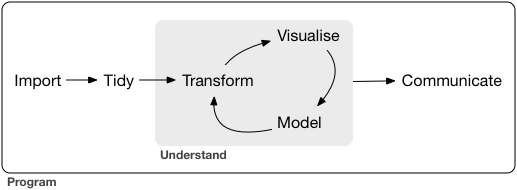
\includegraphics[width=0.6\linewidth]{Imgs/data-science} \end{center}
\end{frame}

\begin{frame}[fragile]{Librerías para cada tarea}
\protect\hypertarget{libreruxedas-para-cada-tarea}{}
\begin{center}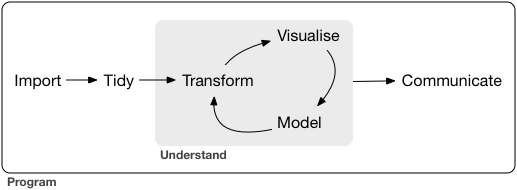
\includegraphics[width=0.3\linewidth]{Imgs/data-science} \end{center}

\begin{itemize}
\tightlist
\item
  \textbf{Import:} \texttt{readr}\\
\item
  \textbf{Tidy:} \texttt{tidyr}\\
\item
  \textbf{Transform:} \texttt{dplyr}, \texttt{forcats},
  \texttt{stringr}\\
\item
  \textbf{Visualize:} \texttt{ggplot2}\\
\item
  \textbf{Model:} \texttt{tidymodels}\\
\item
  \textbf{Communicate:} \texttt{rmarkdown}\\
\item
  \textbf{Program:} \texttt{magrittr}, \texttt{purrr}, \texttt{tibble}
\end{itemize}

Algunos libros:

\begin{itemize}
\tightlist
\item
  \href{https://r4ds.had.co.nz/tidy-data.html}{Wickham/Grolemund
  (2017)}.*
\item
  \href{https://bookdown.org/yihui/rmarkdown/}{Yihui Xie, J. J. Allaire,
  Garrett Grolemund}
\end{itemize}
\end{frame}

\begin{frame}[fragile]{Más sobre \texttt{tidyverse}}
\protect\hypertarget{muxe1s-sobre-tidyverse-1}{}
Lo que se intenta es hacer un diseño y una gramática que sea sencilla
como una API para usuarios no ``tecnólogos''.

\begin{itemize}
\item
  Las \texttt{tibbles} como estructura de datos (superan a los
  \texttt{data.frames} y simplifican los \texttt{data.table})
\item
  El operador \texttt{\%\textgreater{}\%} para crear flujos de datos y
  funciones.
\item
  Estandarizar la nomenclatura de las funciones,
\item
  Establecer un orden razonable en los argumentos de las funciones (por
  ejemplo,
  \texttt{fn(argumento\_A\ =\ datos,\ argumento\_B\ =\ etiquetas\ de\ las\ columnas,\ ...)}.
\end{itemize}
\end{frame}

\begin{frame}[fragile]{Más sobre \texttt{tidyverse}}
\protect\hypertarget{muxe1s-sobre-tidyverse-2}{}
La sintaxis del \texttt{tidyverse} puede verse como un ``dialecto'' de
\texttt{R}.

\begin{center}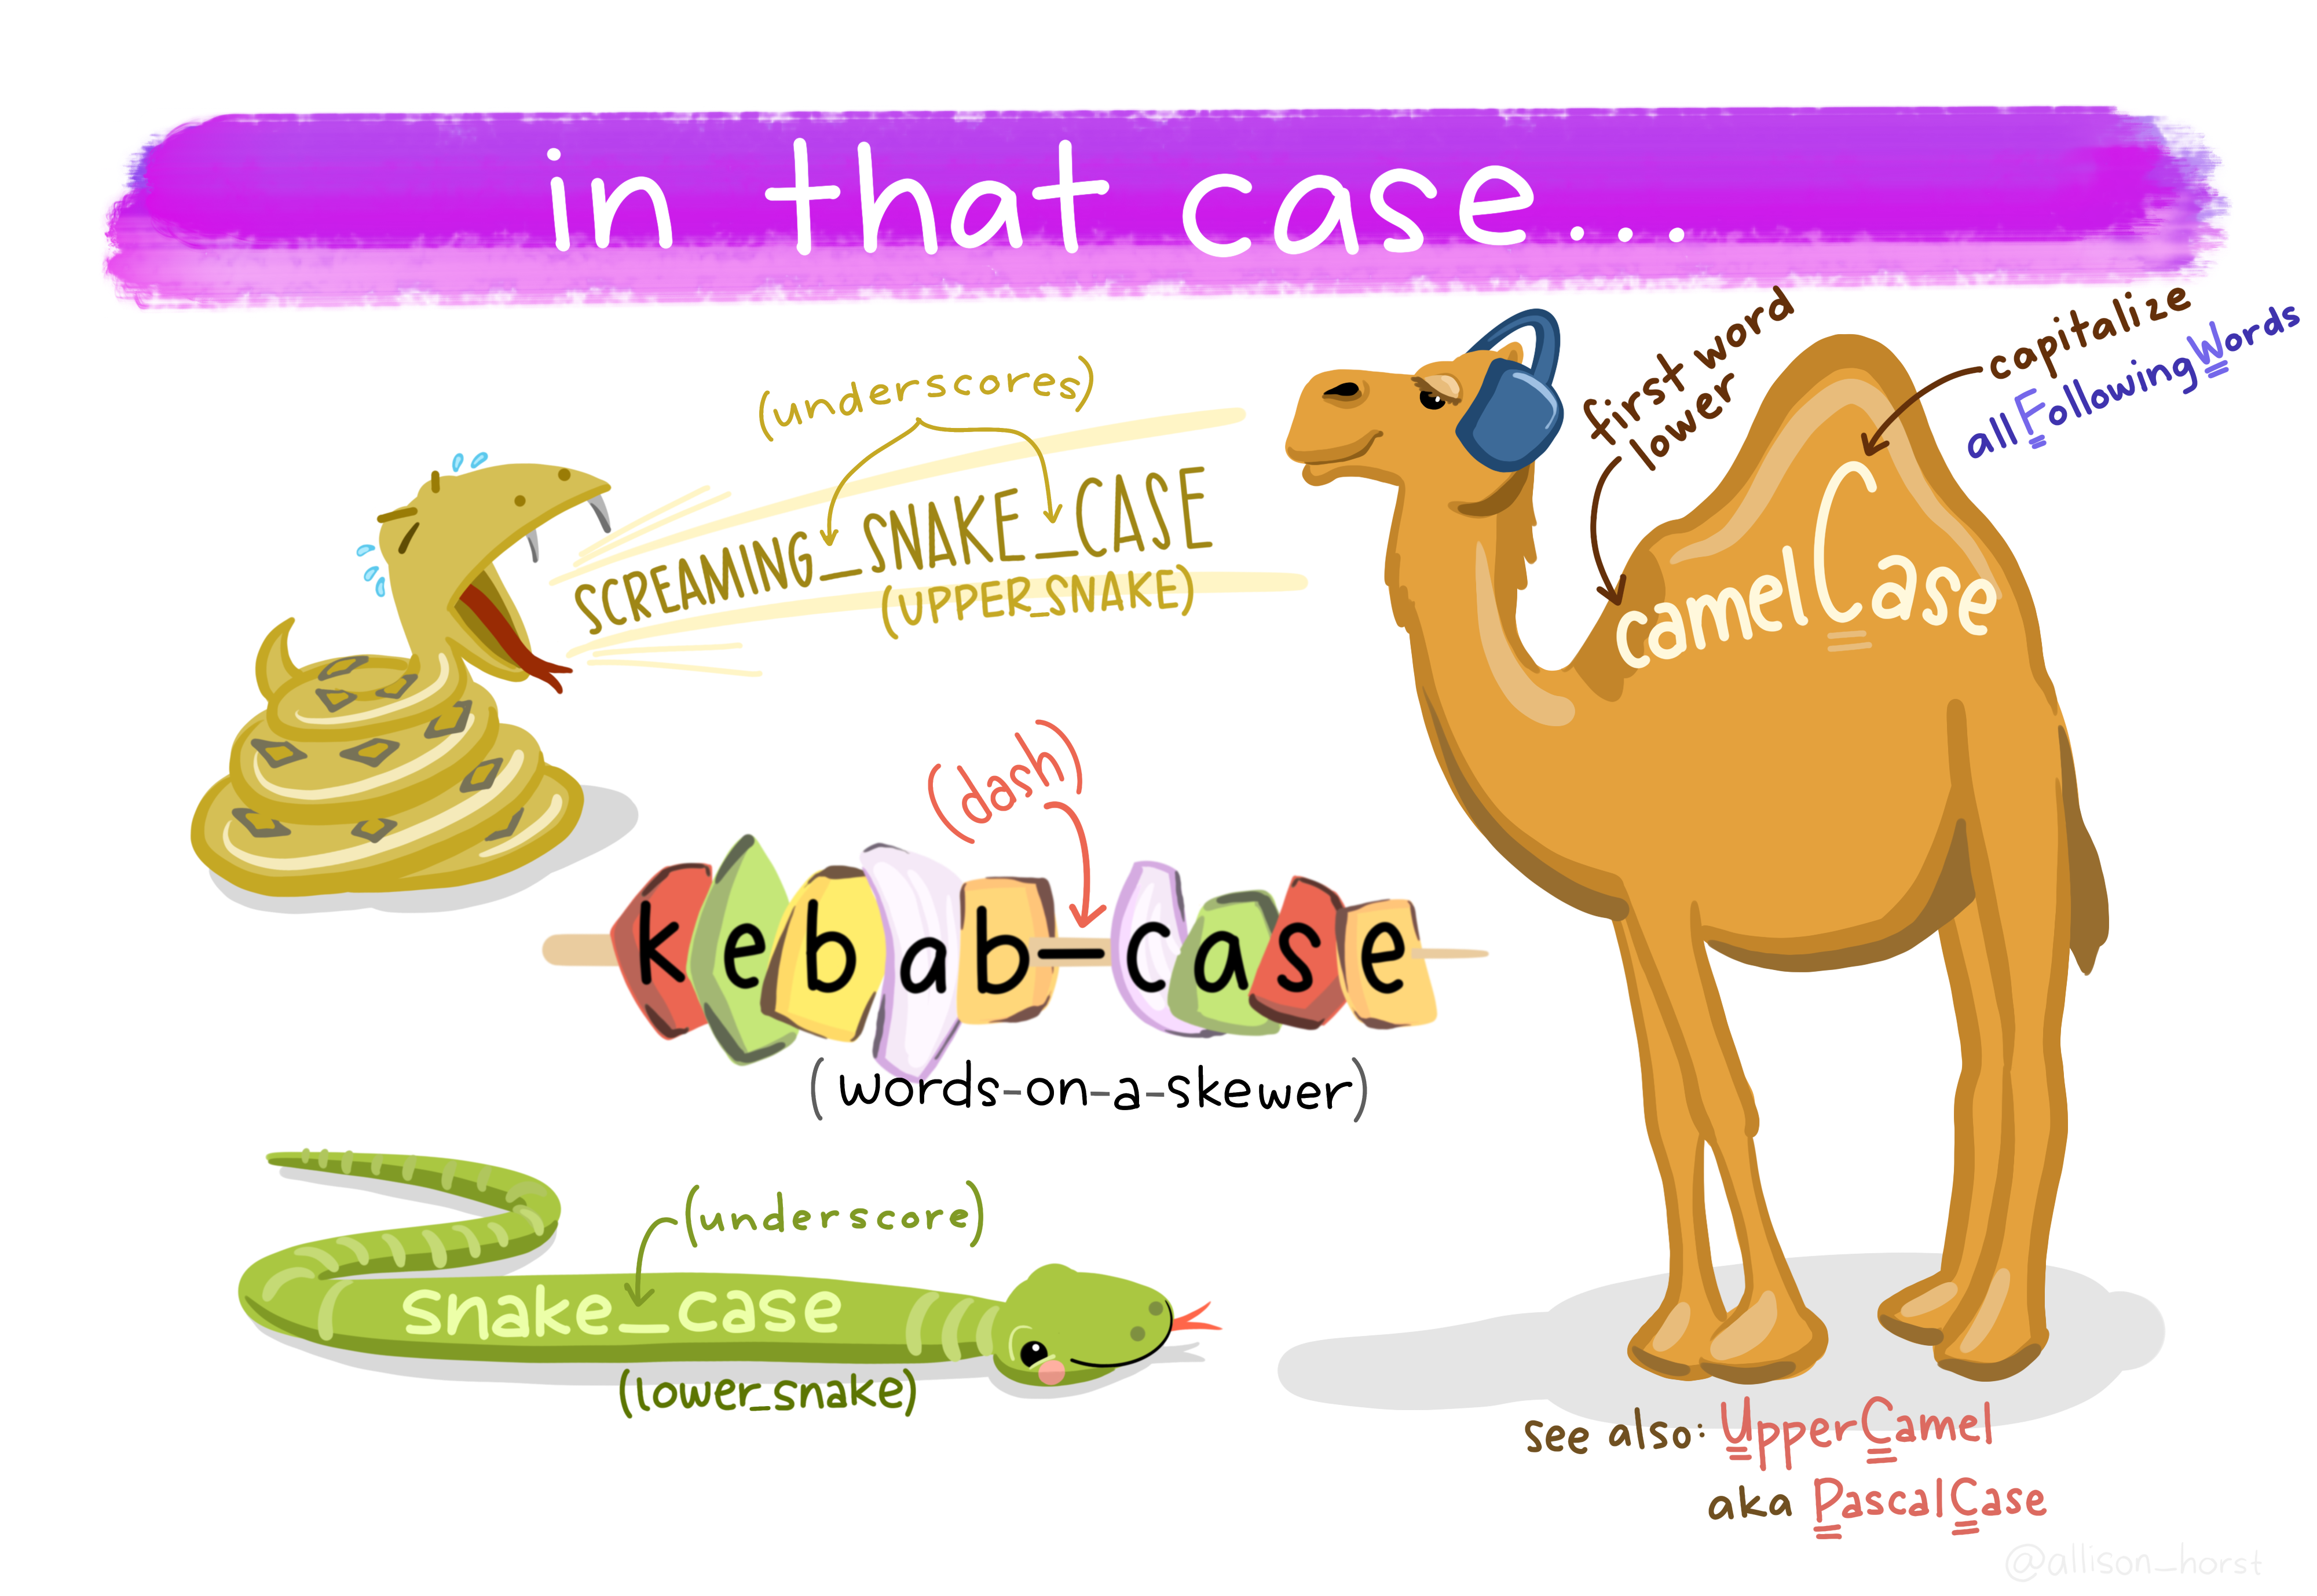
\includegraphics[width=0.4\linewidth]{Imgs/serpiente_camello} \end{center}

\emph{Nota: Para más información}, véase
\href{https://design.tidyverse.org/}{Tidyverse Team (2020)} y
\href{https://cran.r-project.org/web/packages/tidyverse/vignettes/manifesto.html}{Wickham
(2019)}.
\end{frame}

\hypertarget{tidy-data}{%
\section{Tidy data}\label{tidy-data}}

\begin{frame}{¿Qué es tidy data?}
\protect\hypertarget{quuxe9-es-tidy-data}{}
Los conjuntos de datos ordenados son todos iguales; pero cada conjunto
de datos desordenado es desordenado a su manera.
\href{https://r4ds.had.co.nz/tidy-data.html}{Wickham/Grolemund: r4ds}

Si tenemos datos provenientes de distintas fuentes, seguramente
tendremos que estructurarlos en una única tibble.

\textbf{Principios de los datos estructurados:}

El concepto de datos ordenados implica conjuntos de datos rectangulares
y tabulares compuestos por filas y columnas:

\begin{enumerate}
\item
  Cada variable forma una columna.
\item
  Cada observación forma una fila.
\item
  Cada tipo de unidad de observación forma una tabla.
\end{enumerate}
\end{frame}

\begin{frame}{¿Qué es tidy data?}
\protect\hypertarget{quuxe9-es-tidy-data-1}{}
\begin{center}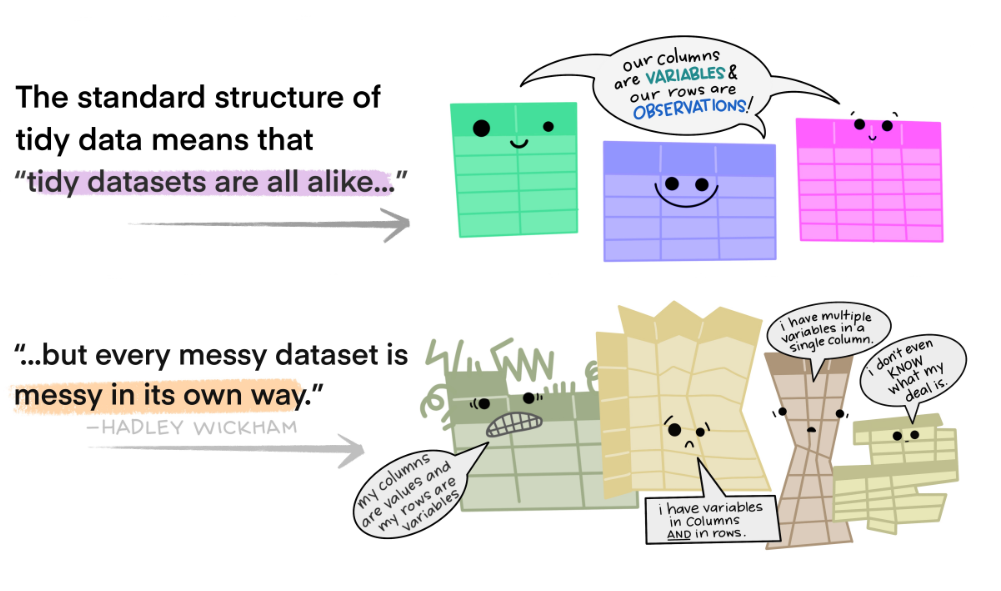
\includegraphics[width=0.6\linewidth]{Imgs/tidy_data} \end{center}
\end{frame}

\begin{frame}{Estructurar y ordenar datos (tidy)}
\protect\hypertarget{estructurar-y-ordenar-datos-tidy}{}
\textbf{Violaciones de los principios de los datos ordenados:}

\begin{enumerate}
\item
  Las cabeceras de las columnas son valores, no nombres de variables.
\item
  Se almacenan múltiples variables en una columna.\\
\item
  Las variables se almacenan tanto en filas como en columnas.
\item
  Se almacenan múltiples tipos de unidades de observación en la misma
  tabla.
\item
  Una misma unidad de observación se almacena en varias tablas.
\end{enumerate}
\end{frame}

\begin{frame}[fragile]{Estructurar y ordenar datos}
\protect\hypertarget{estructurar-y-ordenar-datos}{}
Veamos ejemplos de lo anterior con unos datos de
\href{https://allisonhorst.github.io/palmerpenguins/}{pingüinos} con los
que seguiremos trabajando luego.

\begin{Shaded}
\begin{Highlighting}[]
\CommentTok{\#install.packages("palmerpenguins",dep=TRUE)}
\FunctionTok{library}\NormalTok{(}\StringTok{"palmerpenguins"}\NormalTok{)}
\FunctionTok{print}\NormalTok{(penguins, }\AttributeTok{width =} \DecValTok{50}\NormalTok{)}
\end{Highlighting}
\end{Shaded}

\begin{verbatim}
# A tibble: 344 x 8
   species island    bill_length_mm bill_depth_mm
   <fct>   <fct>              <dbl>         <dbl>
 1 Adelie  Torgersen           39.1          18.7
 2 Adelie  Torgersen           39.5          17.4
 3 Adelie  Torgersen           40.3          18  
 4 Adelie  Torgersen           NA            NA  
 5 Adelie  Torgersen           36.7          19.3
 6 Adelie  Torgersen           39.3          20.6
 7 Adelie  Torgersen           38.9          17.8
 8 Adelie  Torgersen           39.2          19.6
 9 Adelie  Torgersen           34.1          18.1
10 Adelie  Torgersen           42            20.2
# ... with 334 more rows, and 4 more variables:
#   flipper_length_mm <int>, body_mass_g <int>,
#   sex <fct>, year <int>
\end{verbatim}
\end{frame}

\begin{frame}[fragile]{Estructurar y ordenar datos (tidy)}
\protect\hypertarget{estructurar-y-ordenar-datos-tidy-1}{}
\begin{verbatim}
# A tibble: 3 x 4
  species   Biscoe Dream Torgersen
  <fct>      <int> <int>     <int>
1 Adelie        44    56        52
2 Chinstrap     NA    68        NA
3 Gentoo       124    NA        NA
\end{verbatim}

\begin{verbatim}
# A tibble: 5 x 3
  col            island     year
  <chr>          <fct>     <int>
1 Gentoo_NA      Biscoe     2007
2 Adelie_male    Torgersen  2007
3 Gentoo_female  Biscoe     2008
4 Chinstrap_male Dream      2008
5 Adelie_male    Torgersen  2009
\end{verbatim}

\begin{verbatim}
# A tibble: 3 x 4
  term              bill_length_mm bill_depth_mm flipper_length_mm
  <chr>                      <dbl>         <dbl>             <dbl>
1 bill_length_mm            NA            -0.235             0.656
2 bill_depth_mm             -0.235        NA                -0.584
3 flipper_length_mm          0.656        -0.584            NA    
\end{verbatim}
\end{frame}

\begin{frame}[fragile]{Estructurar y ordenar datos (tidy)}
\protect\hypertarget{estructurar-y-ordenar-datos-tidy-2}{}
\begin{verbatim}
# A tibble: 6 x 6
  species   island sex    model              mpg   cyl
  <fct>     <fct>  <fct>  <chr>            <dbl> <dbl>
1 Chinstrap Dream  female <NA>              NA      NA
2 Gentoo    Biscoe female <NA>              NA      NA
3 Gentoo    Biscoe male   <NA>              NA      NA
4 <NA>      <NA>   <NA>   Merc 450SLC       15.2     8
5 <NA>      <NA>   <NA>   Dodge Challenger  15.5     8
6 <NA>      <NA>   <NA>   Pontiac Firebird  19.2     8
\end{verbatim}

\begin{verbatim}
# A tibble: 6 x 6
  species island sex    model               mpg   cyl
  <fct>   <fct>  <fct>  <chr>             <dbl> <dbl>
1 Adelie  Dream  female <NA>               NA      NA
2 Adelie  Dream  female <NA>               NA      NA
3 Gentoo  Biscoe male   <NA>               NA      NA
4 <NA>    <NA>   <NA>   Hornet Sportabout  18.7     8
5 <NA>    <NA>   <NA>   Honda Civic        30.4     4
6 <NA>    <NA>   <NA>   Porsche 914-2      26       4
\end{verbatim}
\end{frame}

\begin{frame}{Estructurar y ordenar datos (tidy)}
\protect\hypertarget{estructurar-y-ordenar-datos-tidy-3}{}
\begin{center}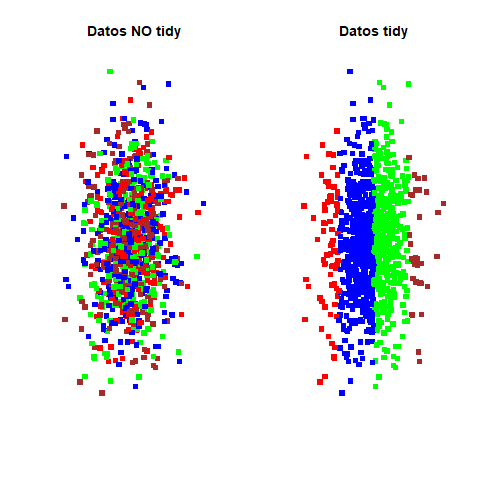
\includegraphics[width=0.5\linewidth]{Imgs/plot_tidy} \end{center}
\end{frame}

\hypertarget{magrittr-pipes-tuberuxedas}{%
\section{Magrittr pipes (tuberías)}\label{magrittr-pipes-tuberuxedas}}

\begin{frame}[fragile]{Datos de los pingüinos del Archipelago de Palmer
(Antarctica)}
\protect\hypertarget{datos-de-los-pinguxfcinos-del-archipelago-de-palmer-antarctica}{}
Como mencionamos antes, para poner ejemplos de los distintos paquetes de
\texttt{tidyverse} utilizamos datos del paquete \texttt{palmerpenguins}
de \href{https://allisonhorst.github.io/palmerpenguins/}{Allison Horst}.

El paquete incluye datos sobre los pingüinos observados en las islas del
archipiélago Palmer, cerca de la estación Palmer, en la Antártida.

\begin{center}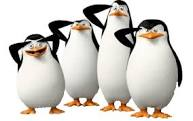
\includegraphics[width=0.3\linewidth]{Imgs/pinguinos_madagascar} \end{center}
\end{frame}

\begin{frame}{Datos de los pingüinos}
\protect\hypertarget{datos-de-los-pinguxfcinos}{}
\begin{center}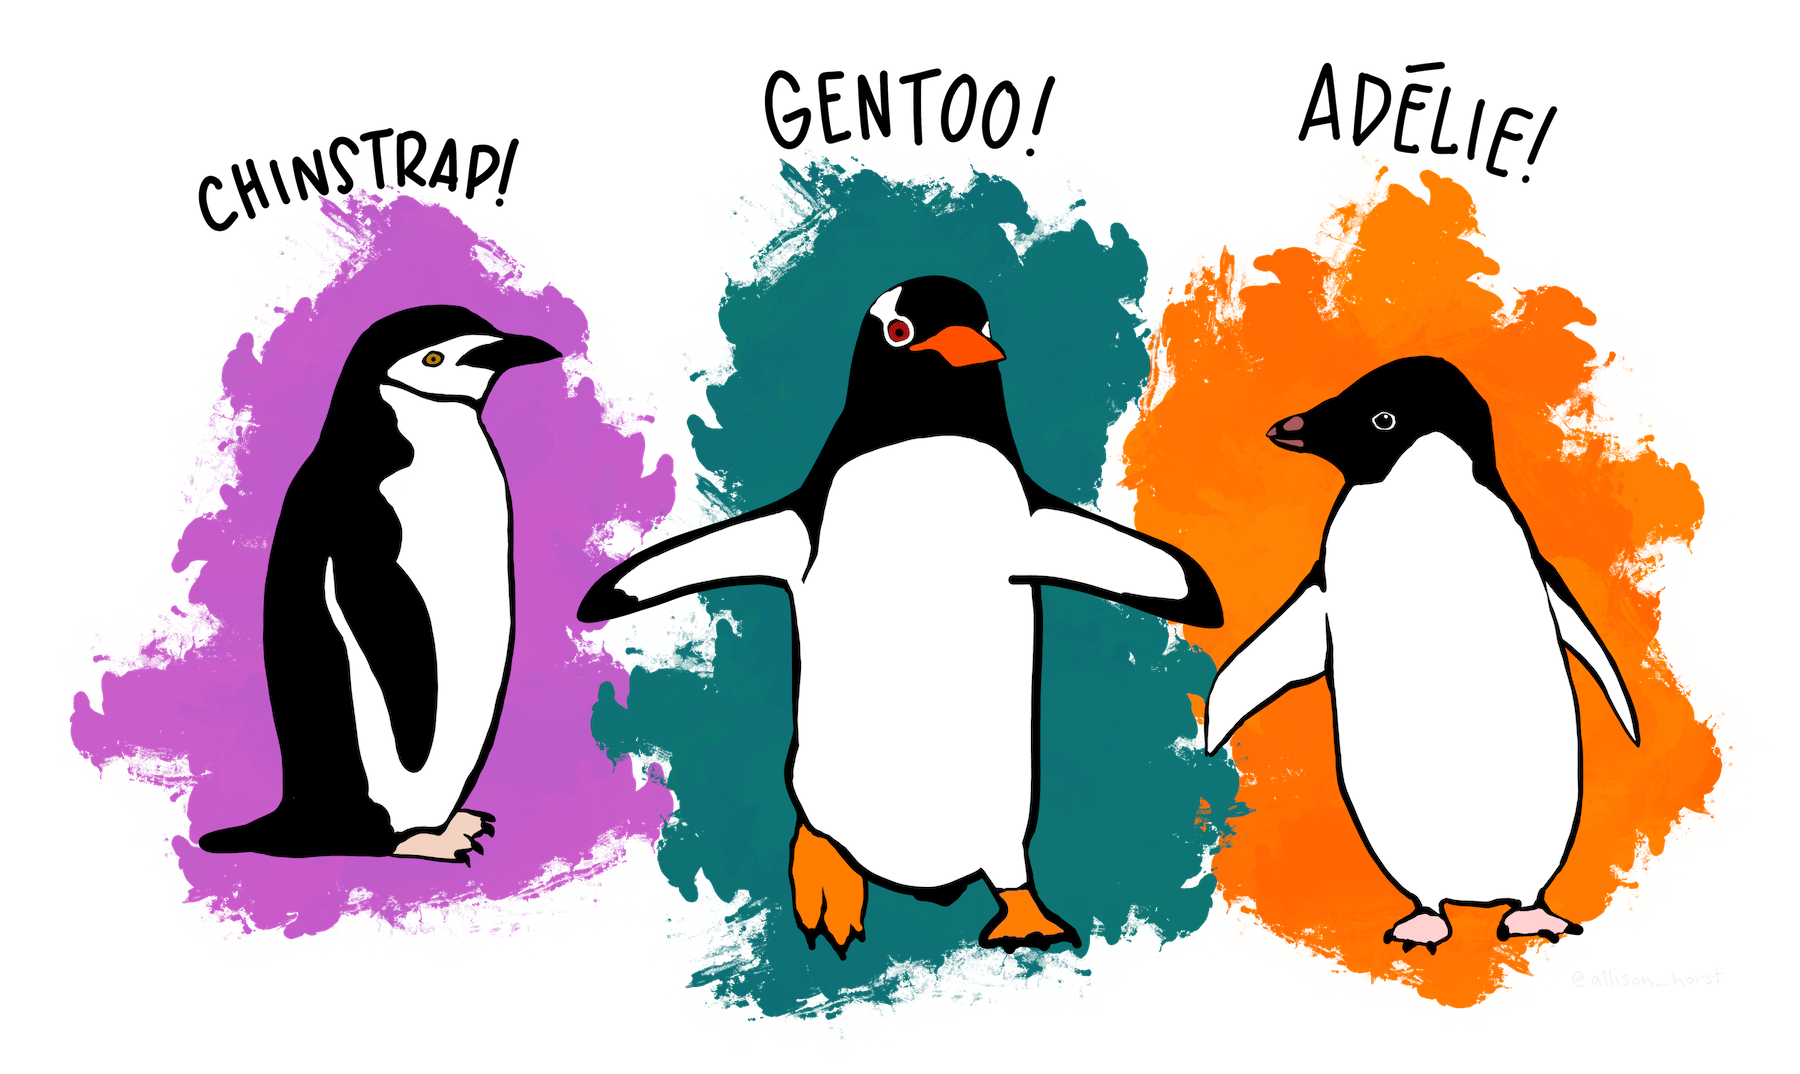
\includegraphics[width=0.35\linewidth]{Imgs/lter_penguins} \end{center}

\begin{center}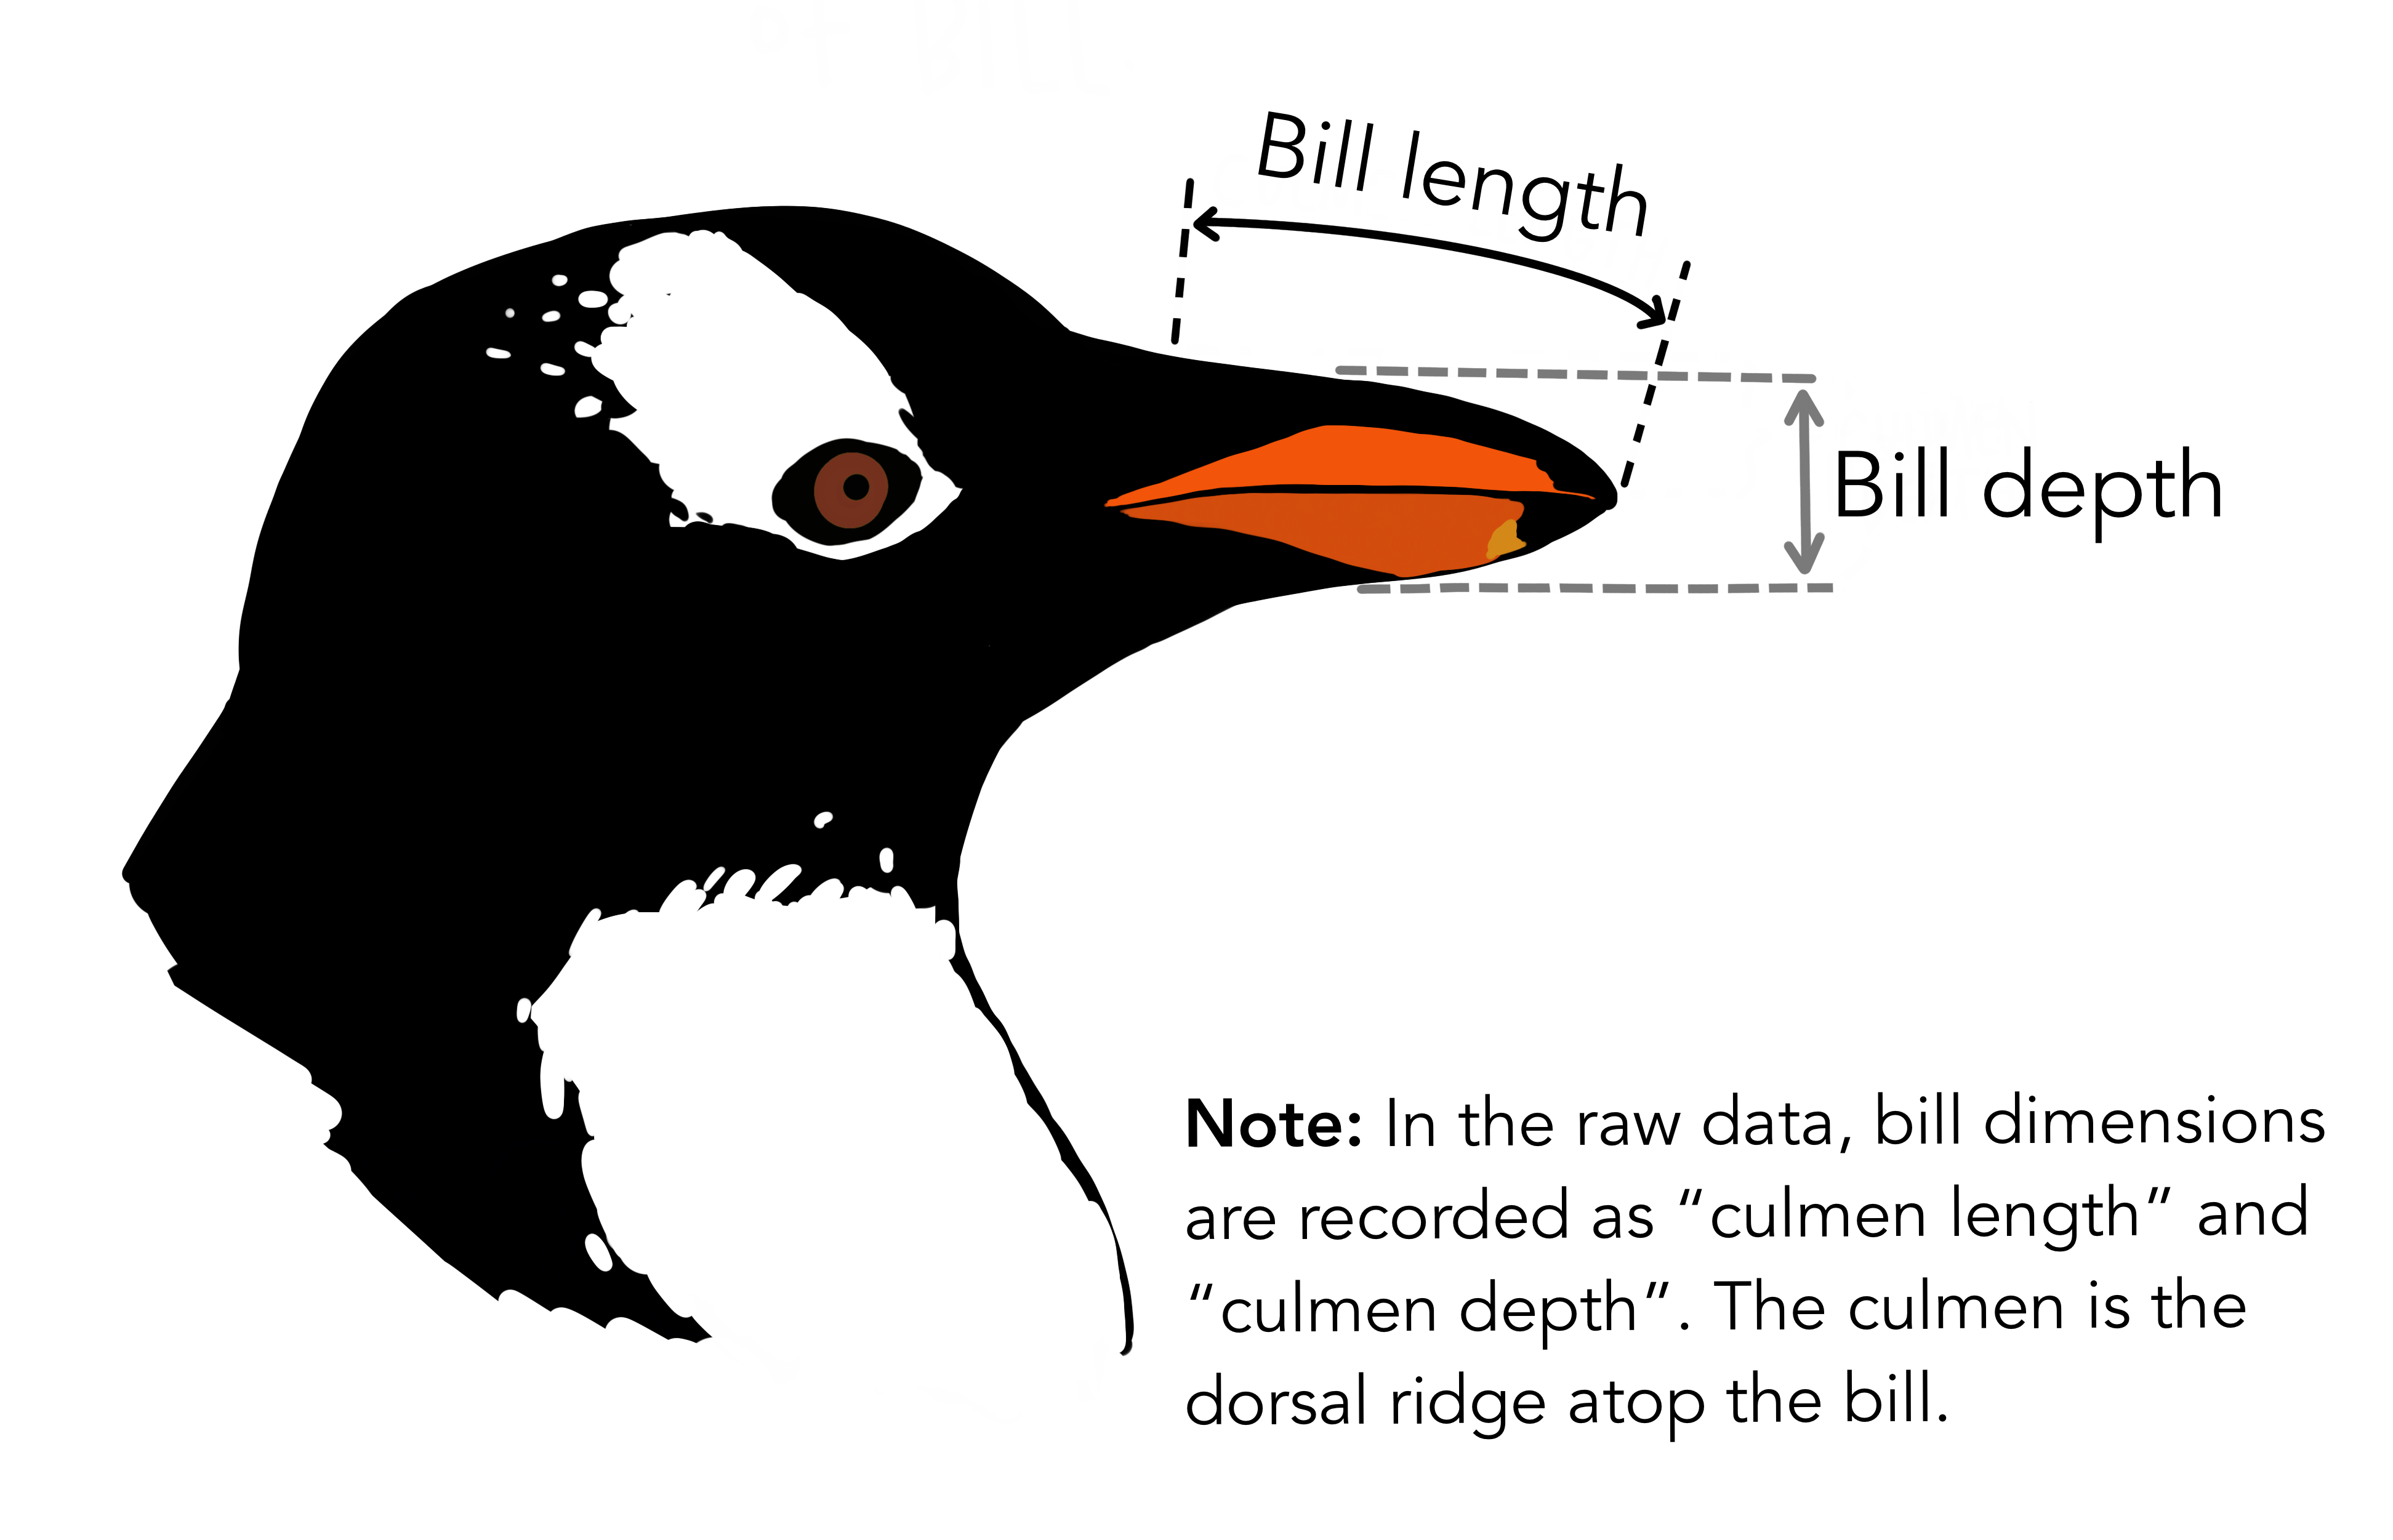
\includegraphics[width=0.35\linewidth]{Imgs/culmen_depth} \end{center}
\end{frame}

\begin{frame}[fragile]{Operadores de ``tuberías'' para \texttt{R}}
\protect\hypertarget{operadores-de-tuberuxedas-para-r}{}
\begin{flushright}
\includegraphics[width=0.05\linewidth]{Imgs/logo_pipe} \end{flushright}

Los operadores pipes de \texttt{magrittr} son:

\begin{itemize}
\tightlist
\item
  \textbf{Operador de tuberías:} \texttt{\%\textgreater{}\%}
\item
  \textbf{Operador de asignación:}
  \texttt{\%\textless{}\textgreater{}\%}
\item
  \textbf{Operador ``T'':} \texttt{\%T\textgreater{}\%}
\item
  \textbf{Operador de extracción (``exposition''):} \texttt{\%\$\%}.
\end{itemize}

\textbf{Ejemplo}

\begin{Shaded}
\begin{Highlighting}[]
\FunctionTok{rnorm}\NormalTok{(}\DecValTok{200}\NormalTok{) }\SpecialCharTok{\%\textgreater{}\%}
\FunctionTok{matrix}\NormalTok{(}\AttributeTok{ncol =} \DecValTok{2}\NormalTok{) }\SpecialCharTok{\%T\textgreater{}\%}
\NormalTok{plot }\SpecialCharTok{\%\textgreater{}\%} \CommentTok{\# plot no suele retornar nada}
\NormalTok{colSums}
\end{Highlighting}
\end{Shaded}
\end{frame}

\begin{frame}[fragile]{Operadores de ``tuberías'' para \texttt{R}}
\protect\hypertarget{operadores-de-tuberuxedas-para-r-1}{}
Estos operadores pretenden mejorar la legibilidad de los códigos de
múltiples maneras:

\begin{itemize}
\item
  Organizando las operaciones en una cadena de instrucciones encadenadas
  (de izquierda a derecha) fácilmente legible,
\item
  Evitando las llamadas a funciones anidadas,
\item
  Minimizando el uso de asignaciones de variables locales
  (\texttt{\textless{}-}) y definiciones de funciones,
\item
  Añadiendo y/o eliminando fácilmente pasos del ``pipeline'' sin romper
  el código.
\end{itemize}

El operador \%\$\% (pasa las variables de una tibble/data.frame.

\begin{Shaded}
\begin{Highlighting}[]
\FunctionTok{library}\NormalTok{(magrittr)}
\NormalTok{iris }\SpecialCharTok{\%\textgreater{}\%}
  \FunctionTok{subset}\NormalTok{(Sepal.Length }\SpecialCharTok{\textgreater{}} \FunctionTok{mean}\NormalTok{(Sepal.Length)) }\SpecialCharTok{\%$\%}
  \FunctionTok{cor}\NormalTok{(Sepal.Length, Sepal.Width)}
\end{Highlighting}
\end{Shaded}
\end{frame}

\begin{frame}[fragile]{Operadores de ``tuberías'' para \texttt{R}}
\protect\hypertarget{operadores-de-tuberuxedas-para-r-2}{}
\begin{Shaded}
\begin{Highlighting}[]
\FunctionTok{library}\NormalTok{(magrittr)}
\FunctionTok{data.frame}\NormalTok{(}\AttributeTok{z =} \FunctionTok{rnorm}\NormalTok{(}\DecValTok{100}\NormalTok{)) }\SpecialCharTok{\%$\%}  \FunctionTok{ts.plot}\NormalTok{(z)}
\end{Highlighting}
\end{Shaded}

\begin{center}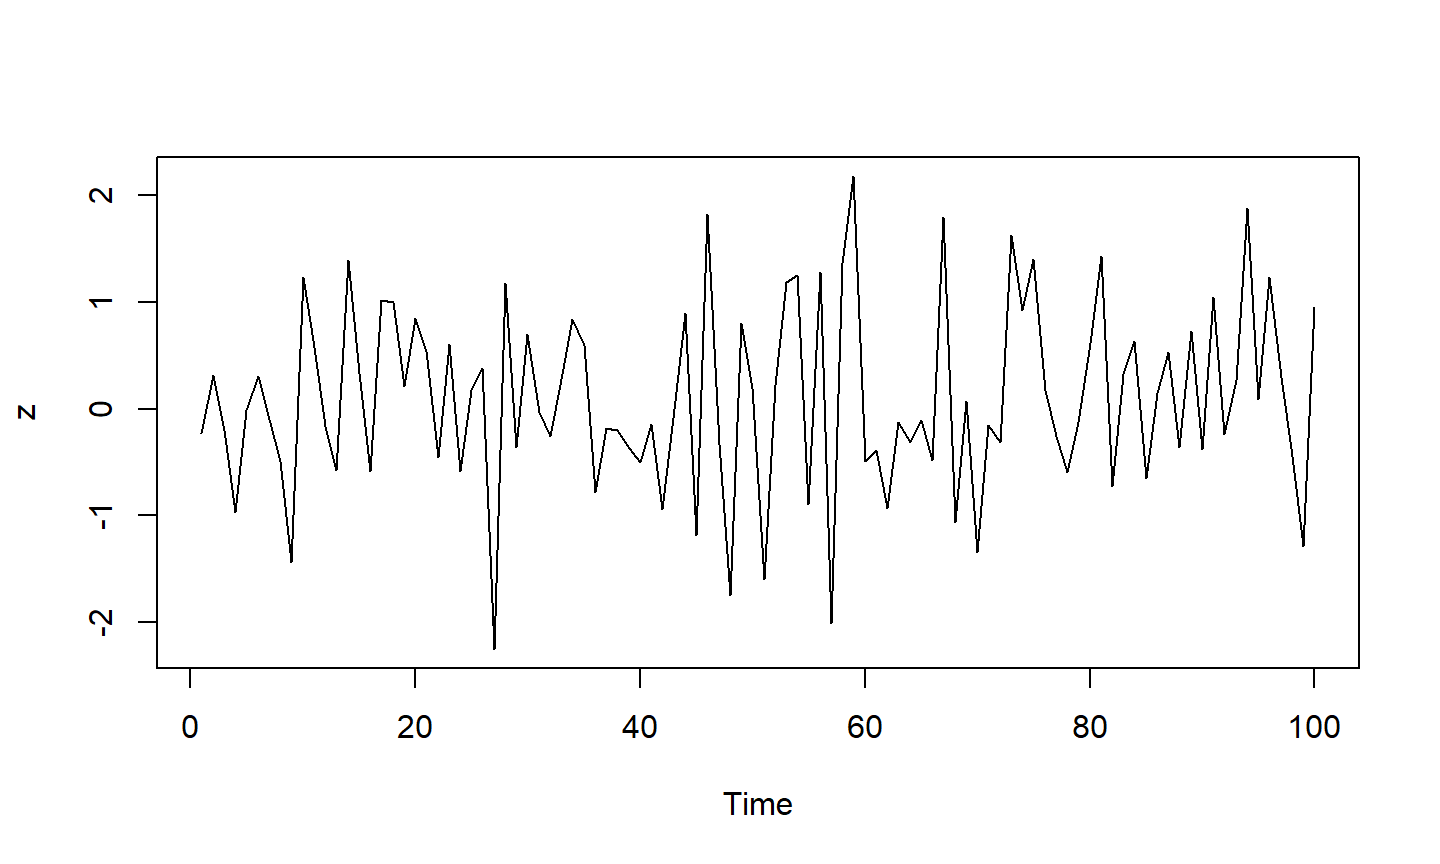
\includegraphics[width=0.5\linewidth]{tidyverse_AD_miércolew_5_oct_files/figure-beamer/unnamed-chunk-17-1} \end{center}
\end{frame}

\begin{frame}[fragile]{El operador pipe}
\protect\hypertarget{el-operador-pipe}{}
\textbf{pipes básicos:} pasan un valor, atributo u objeto (LHS: Left
Hand Side ) a la siguiente llamada de función (RHS: Right Hand Side)
como \textbf{primer} argumento

\begin{Shaded}
\begin{Highlighting}[]
\NormalTok{x }\SpecialCharTok{\%\textgreater{}\%}\NormalTok{ f }\CommentTok{\# equivalente a: f(x)}
\NormalTok{x }\SpecialCharTok{\%\textgreater{}\%} \FunctionTok{f}\NormalTok{(y) }\CommentTok{\# equivalente a: f(x, y)}
\NormalTok{x }\SpecialCharTok{\%\textgreater{}\%}\NormalTok{ f }\SpecialCharTok{\%\textgreater{}\%}\NormalTok{ g }\SpecialCharTok{\%\textgreater{}\%}\NormalTok{ h }\CommentTok{\# equivalente a: h(g(f(x)))}
\end{Highlighting}
\end{Shaded}
\end{frame}

\begin{frame}[fragile]{El operador pipe}
\protect\hypertarget{el-operador-pipe-1}{}
\textbf{pipes con marcadores de posición:} reenvian un valor u objeto
(LHS) a la siguiente llamada de función (RHS) como \textbf{cualquier}
argumento

\begin{Shaded}
\begin{Highlighting}[]
\NormalTok{x }\SpecialCharTok{\%\textgreater{}\%} \FunctionTok{f}\NormalTok{(.) }\CommentTok{\# equivalente a: x \%\textgreater{}\% f}
\NormalTok{x }\SpecialCharTok{\%\textgreater{}\%} \FunctionTok{f}\NormalTok{(y, .) }\CommentTok{\# equivalente a: f(y, x)}
\NormalTok{x }\SpecialCharTok{\%\textgreater{}\%} \FunctionTok{f}\NormalTok{(y, }\AttributeTok{z =}\NormalTok{ .) }\CommentTok{\# equivalente a: f(y, z = x)}
\NormalTok{x }\SpecialCharTok{\%\textgreater{}\%} \FunctionTok{f}\NormalTok{(}\AttributeTok{y =} \FunctionTok{nrow}\NormalTok{(.),}
        \AttributeTok{z =} \FunctionTok{ncol}\NormalTok{(.))  }\CommentTok{\# equivalente a: f(x, y = nrow(x), z = ncol(x))}
\end{Highlighting}
\end{Shaded}
\end{frame}

\begin{frame}[fragile]{Construcción de funciones con pipes}
\protect\hypertarget{construcciuxf3n-de-funciones-con-pipes}{}
Una secuencia de código que comienza con el marcador de posición
(\texttt{.}) devuelve una función que puede utilizarse para aplicar
posteriormente la tubería a valores concretos

\begin{Shaded}
\begin{Highlighting}[]
\NormalTok{f }\OtherTok{\textless{}{-}}\NormalTok{ . }\SpecialCharTok{\%\textgreater{}\%}\NormalTok{ cos }\SpecialCharTok{\%\textgreater{}\%}\NormalTok{ sin }\CommentTok{\# equivalente a: f \textless{}{-} function(.) sin(cos(.))}
\end{Highlighting}
\end{Shaded}

\begin{Shaded}
\begin{Highlighting}[]
\FunctionTok{f}\NormalTok{(}\DecValTok{20}\NormalTok{) }\CommentTok{\# equivalente a: la tubería 20 \%\textgreater{}\% cos \%\textgreater{}\% sin}
\end{Highlighting}
\end{Shaded}

\blue{Nota: Para saber más sobre} \texttt{\%\textgreater{}\%}, haced
\texttt{vignette("magrittr")} en la consola de R.

\red{Se puede obtener la cadena} \texttt{\%\textgreater{}\%} en Rstudio
desktop utilizando el atajo de teclado:

\red{Ctrl + Shift  + M}.
\end{frame}

\begin{frame}[fragile]{Ejemplo con el operador pipe}
\protect\hypertarget{ejemplo-con-el-operador-pipe}{}
\textbf{Pregunta:} ¿Cuál es la masa corporal media en gramos de todos
los pingüinos observados en el año 2007 (tras excluir los valores
perdidos)?

\textbf{En un mundo sin pipes:}

\begin{Shaded}
\begin{Highlighting}[]
\FunctionTok{mean}\NormalTok{(}\FunctionTok{subset}\NormalTok{(penguins, year }\SpecialCharTok{==} \DecValTok{2007}\NormalTok{)}\SpecialCharTok{$}\NormalTok{body\_mass\_g, }\AttributeTok{na.rm =}\NormalTok{ T)}

\CommentTok{\# alternativamente:}
\NormalTok{peng\_bm\_2007 }\OtherTok{\textless{}{-}} \FunctionTok{subset}\NormalTok{(penguins, year }\SpecialCharTok{==} \DecValTok{2007}\NormalTok{)}\SpecialCharTok{$}\NormalTok{body\_mass\_g}
\FunctionTok{media}\NormalTok{(peng\_bm\_2007, }\AttributeTok{na.rm =}\NormalTok{ T)}
\end{Highlighting}
\end{Shaded}

\textbf{En un mundo con pipes:}

\begin{Shaded}
\begin{Highlighting}[]
\NormalTok{penguins }\SpecialCharTok{\%\textgreater{}\%} 
  \FunctionTok{subset}\NormalTok{(year }\SpecialCharTok{==} \DecValTok{2007}\NormalTok{) }\SpecialCharTok{\%\textgreater{}\%} 
\NormalTok{  .}\SpecialCharTok{$}\NormalTok{body\_mass\_g }\SpecialCharTok{\%\textgreater{}\%} 
  \FunctionTok{mean}\NormalTok{(}\AttributeTok{na.rm =}\NormalTok{ T)}
\end{Highlighting}
\end{Shaded}
\end{frame}

\begin{frame}{Ventajas de usar pipes}
\protect\hypertarget{ventajas-de-usar-pipes}{}
\begin{itemize}
\item
  El estilo secuencial de las tuberías mejora la legibilidad y la
  lectura que las funciones anidadas.
\item
  Hace innecesario almacenar los resultados intermedios.
\item
  Es muy fácil añadir o eliminar pasos (empalmes de tuberías)
  individuales en el ``pipe-line/canalización''
\end{itemize}
\end{frame}

\begin{frame}[fragile]{El pipe de R base}
\protect\hypertarget{el-pipe-de-r-base}{}
Las versiones recientes de R ya vienen con un operador de tuberías
nativo también (\texttt{\textbar{}\textgreater{}}).

\begin{Shaded}
\begin{Highlighting}[]
\NormalTok{mtcars }\SpecialCharTok{|\textgreater{}} \FunctionTok{head}\NormalTok{()  }\CommentTok{\#  es lo mismo que head(mtcars)}
\end{Highlighting}
\end{Shaded}

\begin{verbatim}
                   mpg cyl disp  hp drat    wt  qsec vs am gear carb
Mazda RX4         21.0   6  160 110 3.90 2.620 16.46  0  1    4    4
Mazda RX4 Wag     21.0   6  160 110 3.90 2.875 17.02  0  1    4    4
Datsun 710        22.8   4  108  93 3.85 2.320 18.61  1  1    4    1
Hornet 4 Drive    21.4   6  258 110 3.08 3.215 19.44  1  0    3    1
Hornet Sportabout 18.7   8  360 175 3.15 3.440 17.02  0  0    3    2
Valiant           18.1   6  225 105 2.76 3.460 20.22  1  0    3    1
\end{verbatim}

\begin{Shaded}
\begin{Highlighting}[]
\NormalTok{mtcars }\SpecialCharTok{|\textgreater{}} \FunctionTok{head}\NormalTok{(}\DecValTok{2}\NormalTok{) }\CommentTok{\#  es lo mismo que  head(mtcars, 2)}
\end{Highlighting}
\end{Shaded}

\begin{verbatim}
              mpg cyl disp  hp drat    wt  qsec vs am gear carb
Mazda RX4      21   6  160 110  3.9 2.620 16.46  0  1    4    4
Mazda RX4 Wag  21   6  160 110  3.9 2.875 17.02  0  1    4    4
\end{verbatim}

\begin{Shaded}
\begin{Highlighting}[]
\NormalTok{mtcars }\SpecialCharTok{|\textgreater{}} \FunctionTok{subset}\NormalTok{(cyl }\SpecialCharTok{==} \DecValTok{4}\NormalTok{) }\SpecialCharTok{|\textgreater{}} \FunctionTok{nrow}\NormalTok{()  }
\end{Highlighting}
\end{Shaded}

\begin{verbatim}
[1] 11
\end{verbatim}
\end{frame}

\begin{frame}[fragile]{Pipes avanzadas}
\protect\hypertarget{pipes-avanzadas}{}
Los empalmes de tuberías más avanzados como la \texttt{\%T\%} nos
permiten economizar lineas de código.

\begin{itemize}
\tightlist
\item
  \texttt{\%T\textgreater{}\%} se puede utilizar para activar el efecto
  secundario de una función, por ejemplo, para imprimir salidas, y dejar
  que los datos originales pasen por alto el paso respectivo.
\end{itemize}

\begin{Shaded}
\begin{Highlighting}[]
\NormalTok{penguins[}\DecValTok{1}\SpecialCharTok{:}\DecValTok{5}\NormalTok{, }\FunctionTok{c}\NormalTok{(}\StringTok{"island"}\NormalTok{, }\StringTok{"bill\_length\_mm"}\NormalTok{ )] }\SpecialCharTok{\%T\textgreater{}\%} 
\NormalTok{  print }\SpecialCharTok{\%\textgreater{}\%}\NormalTok{ .}\SpecialCharTok{$}\StringTok{"bill\_length\_mm"}  \SpecialCharTok{\%\textgreater{}\%}
  \FunctionTok{mean}\NormalTok{(}\AttributeTok{na.rm=}\NormalTok{T)}
\end{Highlighting}
\end{Shaded}

\begin{verbatim}
# A tibble: 5 x 2
  island    bill_length_mm
  <fct>              <dbl>
1 Torgersen           39.1
2 Torgersen           39.5
3 Torgersen           40.3
4 Torgersen           NA  
5 Torgersen           36.7
\end{verbatim}

\begin{verbatim}
[1] 38.9
\end{verbatim}
\end{frame}

\begin{frame}[fragile]{Tuberías avanzadas}
\protect\hypertarget{tuberuxedas-avanzadas}{}
La pipe \texttt{\%\$\%} extrae las variables del objeto LHS a la
expresión RHS. Es equivalente a:

\begin{Shaded}
\begin{Highlighting}[]
\FunctionTok{plot}\NormalTok{(penguins}\SpecialCharTok{$}\NormalTok{species, penguins}\SpecialCharTok{$}\NormalTok{bill\_length\_mm)}
\end{Highlighting}
\end{Shaded}

\begin{Shaded}
\begin{Highlighting}[]
\NormalTok{penguins }\SpecialCharTok{\%$\%} 
  \FunctionTok{plot}\NormalTok{(species,bill\_length\_mm) }
\end{Highlighting}
\end{Shaded}

\begin{center}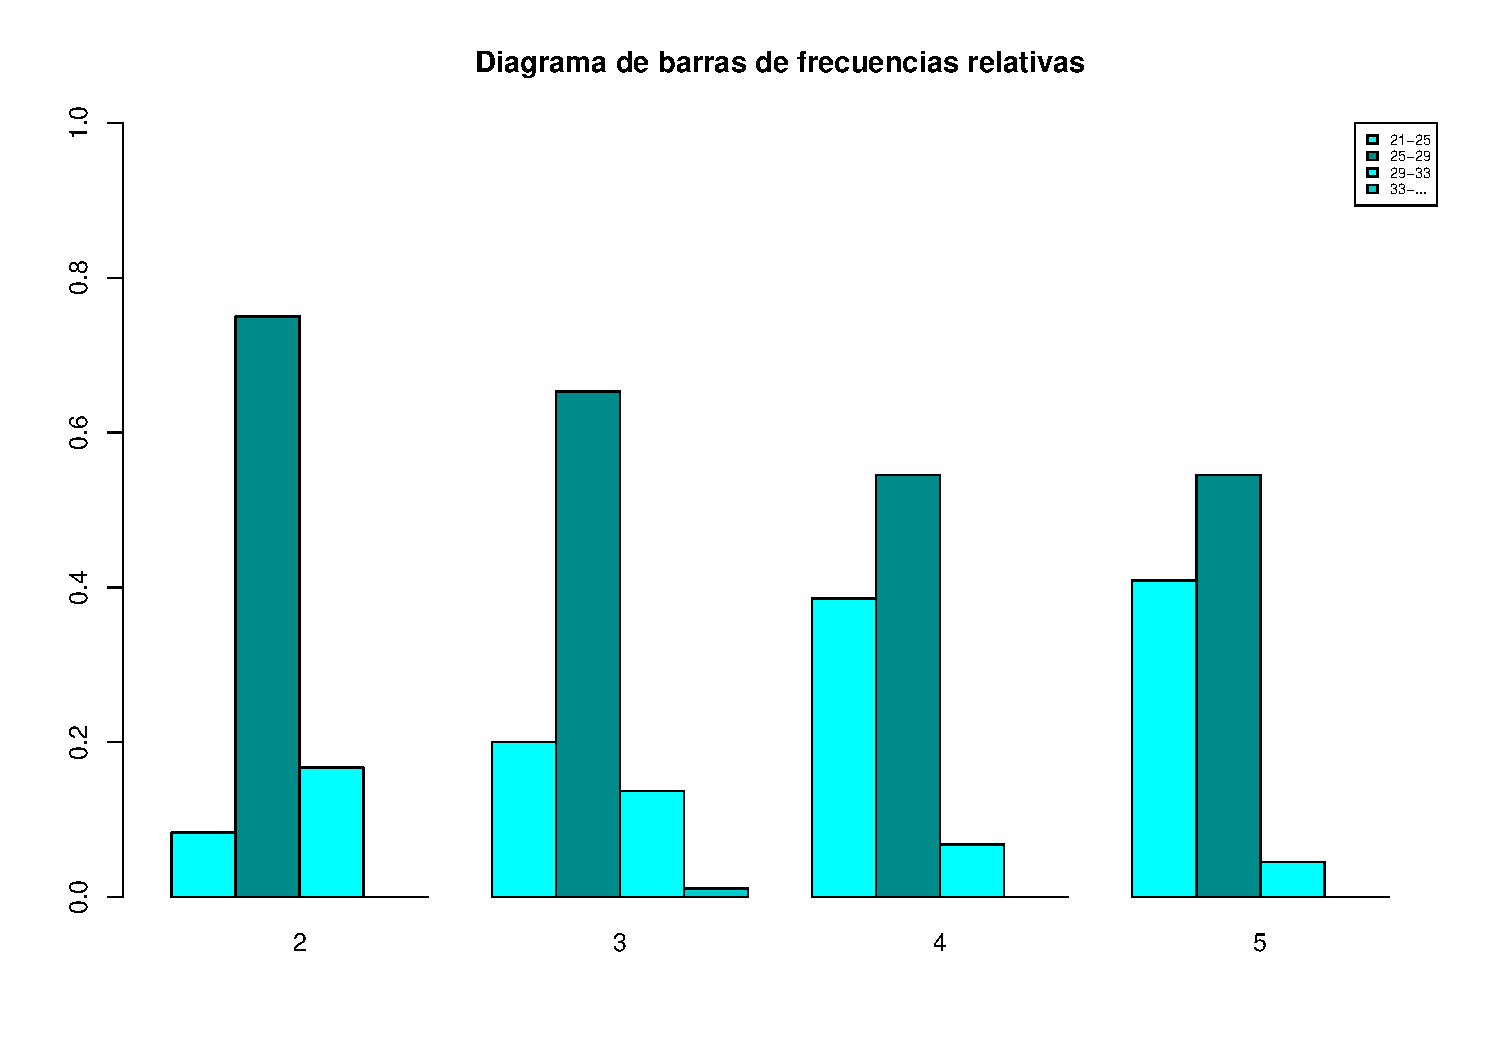
\includegraphics[width=0.5\linewidth]{tidyverse_AD_miércolew_5_oct_files/figure-beamer/unnamed-chunk-27-1} \end{center}
\end{frame}

\begin{frame}[fragile]{Tuberías avanzadas}
\protect\hypertarget{tuberuxedas-avanzadas-1}{}
El operador \texttt{\%\textless{}\textgreater{}\%} se puede utilizar de
forma equivalente al operador de asignación de \texttt{R} base:
(\texttt{\textless{}-}).

Reasigna el resultado de la tubería a la variable inicial.

\hfill\break

\begin{Shaded}
\begin{Highlighting}[]
\NormalTok{variable }\OtherTok{\textless{}{-}}\NormalTok{ penguins}\SpecialCharTok{$}\NormalTok{bill\_length\_mm}
\NormalTok{variable }\SpecialCharTok{\%\textless{}\textgreater{}\%} \FunctionTok{mean}\NormalTok{(}\AttributeTok{na.rm=}\NormalTok{T)}
\NormalTok{variable}
\end{Highlighting}
\end{Shaded}

{[}1{]} 43.92193
\end{frame}

\hypertarget{paquete-tibble}{%
\section{Paquete tibble}\label{paquete-tibble}}

\begin{frame}[fragile]{Data frame avanzado: tibble}
\protect\hypertarget{data-frame-avanzado-tibble}{}
EL paquete \texttt{tibble} proporciona un objeto de tipo data frame
mejorado: \texttt{tbl\_df}. Un \texttt{tibble} se puede crear de cuatro
maneras diferentes.

\begin{enumerate}
\tightlist
\item
  A partir de vectores de columna con \texttt{tibble()}.
\end{enumerate}

\begin{Shaded}
\begin{Highlighting}[]
\FunctionTok{tibble}\NormalTok{(}
  \AttributeTok{x =} \FunctionTok{c}\NormalTok{(}\StringTok{"a"}\NormalTok{, }\StringTok{"b"}\NormalTok{),}
  \AttributeTok{y =} \FunctionTok{c}\NormalTok{(}\DecValTok{1}\NormalTok{, }\DecValTok{2}\NormalTok{),}
  \AttributeTok{z =} \FunctionTok{c}\NormalTok{(T, F)}
\NormalTok{)}
\end{Highlighting}
\end{Shaded}

\begin{verbatim}
# A tibble: 2 x 3
  x         y z    
  <chr> <dbl> <lgl>
1 a         1 TRUE 
2 b         2 FALSE
\end{verbatim}
\end{frame}

\begin{frame}[fragile]{Data frame avanzado: tibble}
\protect\hypertarget{data-frame-avanzado-tibble-1}{}
\begin{enumerate}
\setcounter{enumi}{1}
\tightlist
\item
  Escribiendo en texto por columnas \texttt{tibble}, fila por fila con
  \texttt{tribble()}.
\end{enumerate}

\begin{Shaded}
\begin{Highlighting}[]
\FunctionTok{tribble}\NormalTok{(}
  \SpecialCharTok{\textasciitilde{}}\NormalTok{x, }\SpecialCharTok{\textasciitilde{}}\NormalTok{y, }\SpecialCharTok{\textasciitilde{}}\NormalTok{z,}
  \StringTok{"a"}\NormalTok{, }\DecValTok{1}\NormalTok{, T,}
  \StringTok{"b"}\NormalTok{, }\DecValTok{2}\NormalTok{, F}
\NormalTok{)}
\end{Highlighting}
\end{Shaded}

\begin{verbatim}
# A tibble: 2 x 3
  x         y z    
  <chr> <dbl> <lgl>
1 a         1 TRUE 
2 b         2 FALSE
\end{verbatim}
\end{frame}

\begin{frame}[fragile]{Data frame avanzado: tibble}
\protect\hypertarget{data-frame-avanzado-tibble-2}{}
\begin{enumerate}
\setcounter{enumi}{2}
\tightlist
\item
  Crear un \texttt{tibble} a partir de otro objeto de las clases
  \texttt{matrix} o data.frame\texttt{con}as\_tibble()`.
\end{enumerate}

\begin{Shaded}
\begin{Highlighting}[]
\FunctionTok{data.frame}\NormalTok{(}
  \AttributeTok{x =} \FunctionTok{c}\NormalTok{(}\StringTok{"a"}\NormalTok{, }\StringTok{"b"}\NormalTok{),}
  \AttributeTok{y =} \FunctionTok{c}\NormalTok{(}\DecValTok{1}\NormalTok{, }\DecValTok{2}\NormalTok{),}
  \AttributeTok{z =} \FunctionTok{c}\NormalTok{(T, F)}
\NormalTok{) }\SpecialCharTok{\%\textgreater{}\%} 
\NormalTok{as\_tibble}
\end{Highlighting}
\end{Shaded}

\begin{verbatim}
# A tibble: 2 x 3
  x         y z    
  <chr> <dbl> <lgl>
1 a         1 TRUE 
2 b         2 FALSE
\end{verbatim}
\end{frame}

\begin{frame}[fragile]{Data frame avanzado: tibble}
\protect\hypertarget{data-frame-avanzado-tibble-3}{}
\begin{enumerate}
\setcounter{enumi}{3}
\tightlist
\item
  A partir de vectores con nombre con \texttt{enframe()}.
\end{enumerate}

\begin{Shaded}
\begin{Highlighting}[]
\FunctionTok{c}\NormalTok{(}\AttributeTok{x =} \StringTok{"a"}\NormalTok{, }\AttributeTok{y =} \StringTok{"b"}\NormalTok{, }\AttributeTok{z =} \DecValTok{1}\NormalTok{) }\SpecialCharTok{\%\textgreater{}\%}
  \FunctionTok{enframe}\NormalTok{(}\AttributeTok{name =} \StringTok{"x"}\NormalTok{, }\AttributeTok{value =} \StringTok{"y"}\NormalTok{)}
\end{Highlighting}
\end{Shaded}

\begin{verbatim}
# A tibble: 3 x 2
  x     y    
  <chr> <chr>
1 x     a    
2 y     b    
3 z     1    
\end{verbatim}
\end{frame}

\begin{frame}[fragile]{Data frame avanzado tibble}
\protect\hypertarget{data-frame-avanzado-tibble-4}{}
\red{Diferencias entre tibble y data.frame}

\begin{itemize}
\item
  Un tibble nunca cambia el tipo de entrada.

  \begin{itemize}
  \tightlist
  \item
    Ya no hay que preocuparse de que los caracteres se conviertan
    automáticamente en cadenas.
  \end{itemize}
\item
  Un tibble puede tener columnas que son listas.
\item
  Un tibble puede tener nombres de variables no estándar.

  \begin{itemize}
  \tightlist
  \item
    Pueden empezar por un número o contener espacios.
  \item
    Para utilizarlo se refiere a estos en un backtick:
    \texttt{peso\ en\ Kg}.
  \end{itemize}
\item
  Sólo recicla vectores de longitud 1.
\item
  No tiene como atributo nombres de filas \texttt{row.names}.
\end{itemize}
\end{frame}

\begin{frame}[fragile]{Data frame avanzado tibble}
\protect\hypertarget{data-frame-avanzado-tibble-5}{}
\textbf{Impresión:} Por defecto, \texttt{tibble()} imprime sólo las diez
primeras filas y todas las columnas que caben en la pantalla, y las
clases de las columnas

\begin{Shaded}
\begin{Highlighting}[]
\NormalTok{penguins}
\end{Highlighting}
\end{Shaded}

\begin{verbatim}
# A tibble: 344 x 8
   species island    bill_length_mm bill_depth_mm flipper_length_mm body_mass_g
   <fct>   <fct>              <dbl>         <dbl>             <int>       <int>
 1 Adelie  Torgersen           39.1          18.7               181        3750
 2 Adelie  Torgersen           39.5          17.4               186        3800
 3 Adelie  Torgersen           40.3          18                 195        3250
 4 Adelie  Torgersen           NA            NA                  NA          NA
 5 Adelie  Torgersen           36.7          19.3               193        3450
 6 Adelie  Torgersen           39.3          20.6               190        3650
 7 Adelie  Torgersen           38.9          17.8               181        3625
 8 Adelie  Torgersen           39.2          19.6               195        4675
 9 Adelie  Torgersen           34.1          18.1               193        3475
10 Adelie  Torgersen           42            20.2               190        4250
# ... with 334 more rows, and 2 more variables: sex <fct>, year <int>
\end{verbatim}
\end{frame}

\begin{frame}[fragile]{Data frame avanzado: tibble}
\protect\hypertarget{data-frame-avanzado-tibble-6}{}
Aquí se ve la diferencia con la clase \texttt{data.frame}.

\begin{Shaded}
\begin{Highlighting}[]
\FunctionTok{data.frame}\NormalTok{(penguins)}
\end{Highlighting}
\end{Shaded}

\begin{verbatim}
      species    island bill_length_mm bill_depth_mm flipper_length_mm
1      Adelie Torgersen           39.1          18.7               181
2      Adelie Torgersen           39.5          17.4               186
3      Adelie Torgersen           40.3          18.0               195
4      Adelie Torgersen             NA            NA                NA
5      Adelie Torgersen           36.7          19.3               193
6      Adelie Torgersen           39.3          20.6               190
7      Adelie Torgersen           38.9          17.8               181
8      Adelie Torgersen           39.2          19.6               195
9      Adelie Torgersen           34.1          18.1               193
10     Adelie Torgersen           42.0          20.2               190
11     Adelie Torgersen           37.8          17.1               186
12     Adelie Torgersen           37.8          17.3               180
13     Adelie Torgersen           41.1          17.6               182
14     Adelie Torgersen           38.6          21.2               191
15     Adelie Torgersen           34.6          21.1               198
16     Adelie Torgersen           36.6          17.8               185
17     Adelie Torgersen           38.7          19.0               195
18     Adelie Torgersen           42.5          20.7               197
19     Adelie Torgersen           34.4          18.4               184
20     Adelie Torgersen           46.0          21.5               194
21     Adelie    Biscoe           37.8          18.3               174
22     Adelie    Biscoe           37.7          18.7               180
23     Adelie    Biscoe           35.9          19.2               189
24     Adelie    Biscoe           38.2          18.1               185
25     Adelie    Biscoe           38.8          17.2               180
26     Adelie    Biscoe           35.3          18.9               187
27     Adelie    Biscoe           40.6          18.6               183
28     Adelie    Biscoe           40.5          17.9               187
29     Adelie    Biscoe           37.9          18.6               172
30     Adelie    Biscoe           40.5          18.9               180
31     Adelie     Dream           39.5          16.7               178
32     Adelie     Dream           37.2          18.1               178
33     Adelie     Dream           39.5          17.8               188
34     Adelie     Dream           40.9          18.9               184
35     Adelie     Dream           36.4          17.0               195
36     Adelie     Dream           39.2          21.1               196
37     Adelie     Dream           38.8          20.0               190
38     Adelie     Dream           42.2          18.5               180
39     Adelie     Dream           37.6          19.3               181
40     Adelie     Dream           39.8          19.1               184
41     Adelie     Dream           36.5          18.0               182
42     Adelie     Dream           40.8          18.4               195
43     Adelie     Dream           36.0          18.5               186
44     Adelie     Dream           44.1          19.7               196
45     Adelie     Dream           37.0          16.9               185
46     Adelie     Dream           39.6          18.8               190
47     Adelie     Dream           41.1          19.0               182
48     Adelie     Dream           37.5          18.9               179
49     Adelie     Dream           36.0          17.9               190
50     Adelie     Dream           42.3          21.2               191
51     Adelie    Biscoe           39.6          17.7               186
52     Adelie    Biscoe           40.1          18.9               188
53     Adelie    Biscoe           35.0          17.9               190
54     Adelie    Biscoe           42.0          19.5               200
55     Adelie    Biscoe           34.5          18.1               187
56     Adelie    Biscoe           41.4          18.6               191
57     Adelie    Biscoe           39.0          17.5               186
58     Adelie    Biscoe           40.6          18.8               193
59     Adelie    Biscoe           36.5          16.6               181
60     Adelie    Biscoe           37.6          19.1               194
61     Adelie    Biscoe           35.7          16.9               185
62     Adelie    Biscoe           41.3          21.1               195
63     Adelie    Biscoe           37.6          17.0               185
64     Adelie    Biscoe           41.1          18.2               192
65     Adelie    Biscoe           36.4          17.1               184
66     Adelie    Biscoe           41.6          18.0               192
67     Adelie    Biscoe           35.5          16.2               195
68     Adelie    Biscoe           41.1          19.1               188
69     Adelie Torgersen           35.9          16.6               190
70     Adelie Torgersen           41.8          19.4               198
71     Adelie Torgersen           33.5          19.0               190
72     Adelie Torgersen           39.7          18.4               190
73     Adelie Torgersen           39.6          17.2               196
74     Adelie Torgersen           45.8          18.9               197
75     Adelie Torgersen           35.5          17.5               190
76     Adelie Torgersen           42.8          18.5               195
77     Adelie Torgersen           40.9          16.8               191
78     Adelie Torgersen           37.2          19.4               184
79     Adelie Torgersen           36.2          16.1               187
80     Adelie Torgersen           42.1          19.1               195
81     Adelie Torgersen           34.6          17.2               189
82     Adelie Torgersen           42.9          17.6               196
83     Adelie Torgersen           36.7          18.8               187
84     Adelie Torgersen           35.1          19.4               193
85     Adelie     Dream           37.3          17.8               191
86     Adelie     Dream           41.3          20.3               194
87     Adelie     Dream           36.3          19.5               190
88     Adelie     Dream           36.9          18.6               189
89     Adelie     Dream           38.3          19.2               189
90     Adelie     Dream           38.9          18.8               190
91     Adelie     Dream           35.7          18.0               202
92     Adelie     Dream           41.1          18.1               205
93     Adelie     Dream           34.0          17.1               185
94     Adelie     Dream           39.6          18.1               186
95     Adelie     Dream           36.2          17.3               187
96     Adelie     Dream           40.8          18.9               208
97     Adelie     Dream           38.1          18.6               190
98     Adelie     Dream           40.3          18.5               196
99     Adelie     Dream           33.1          16.1               178
100    Adelie     Dream           43.2          18.5               192
101    Adelie    Biscoe           35.0          17.9               192
102    Adelie    Biscoe           41.0          20.0               203
103    Adelie    Biscoe           37.7          16.0               183
104    Adelie    Biscoe           37.8          20.0               190
105    Adelie    Biscoe           37.9          18.6               193
106    Adelie    Biscoe           39.7          18.9               184
107    Adelie    Biscoe           38.6          17.2               199
108    Adelie    Biscoe           38.2          20.0               190
109    Adelie    Biscoe           38.1          17.0               181
110    Adelie    Biscoe           43.2          19.0               197
111    Adelie    Biscoe           38.1          16.5               198
112    Adelie    Biscoe           45.6          20.3               191
113    Adelie    Biscoe           39.7          17.7               193
114    Adelie    Biscoe           42.2          19.5               197
115    Adelie    Biscoe           39.6          20.7               191
116    Adelie    Biscoe           42.7          18.3               196
117    Adelie Torgersen           38.6          17.0               188
118    Adelie Torgersen           37.3          20.5               199
119    Adelie Torgersen           35.7          17.0               189
120    Adelie Torgersen           41.1          18.6               189
121    Adelie Torgersen           36.2          17.2               187
122    Adelie Torgersen           37.7          19.8               198
123    Adelie Torgersen           40.2          17.0               176
124    Adelie Torgersen           41.4          18.5               202
125    Adelie Torgersen           35.2          15.9               186
126    Adelie Torgersen           40.6          19.0               199
127    Adelie Torgersen           38.8          17.6               191
128    Adelie Torgersen           41.5          18.3               195
129    Adelie Torgersen           39.0          17.1               191
130    Adelie Torgersen           44.1          18.0               210
131    Adelie Torgersen           38.5          17.9               190
132    Adelie Torgersen           43.1          19.2               197
133    Adelie     Dream           36.8          18.5               193
134    Adelie     Dream           37.5          18.5               199
135    Adelie     Dream           38.1          17.6               187
136    Adelie     Dream           41.1          17.5               190
137    Adelie     Dream           35.6          17.5               191
138    Adelie     Dream           40.2          20.1               200
139    Adelie     Dream           37.0          16.5               185
140    Adelie     Dream           39.7          17.9               193
141    Adelie     Dream           40.2          17.1               193
142    Adelie     Dream           40.6          17.2               187
143    Adelie     Dream           32.1          15.5               188
144    Adelie     Dream           40.7          17.0               190
145    Adelie     Dream           37.3          16.8               192
146    Adelie     Dream           39.0          18.7               185
147    Adelie     Dream           39.2          18.6               190
148    Adelie     Dream           36.6          18.4               184
149    Adelie     Dream           36.0          17.8               195
150    Adelie     Dream           37.8          18.1               193
151    Adelie     Dream           36.0          17.1               187
152    Adelie     Dream           41.5          18.5               201
153    Gentoo    Biscoe           46.1          13.2               211
154    Gentoo    Biscoe           50.0          16.3               230
155    Gentoo    Biscoe           48.7          14.1               210
156    Gentoo    Biscoe           50.0          15.2               218
157    Gentoo    Biscoe           47.6          14.5               215
158    Gentoo    Biscoe           46.5          13.5               210
159    Gentoo    Biscoe           45.4          14.6               211
160    Gentoo    Biscoe           46.7          15.3               219
161    Gentoo    Biscoe           43.3          13.4               209
162    Gentoo    Biscoe           46.8          15.4               215
163    Gentoo    Biscoe           40.9          13.7               214
164    Gentoo    Biscoe           49.0          16.1               216
165    Gentoo    Biscoe           45.5          13.7               214
166    Gentoo    Biscoe           48.4          14.6               213
167    Gentoo    Biscoe           45.8          14.6               210
168    Gentoo    Biscoe           49.3          15.7               217
169    Gentoo    Biscoe           42.0          13.5               210
170    Gentoo    Biscoe           49.2          15.2               221
171    Gentoo    Biscoe           46.2          14.5               209
172    Gentoo    Biscoe           48.7          15.1               222
173    Gentoo    Biscoe           50.2          14.3               218
174    Gentoo    Biscoe           45.1          14.5               215
175    Gentoo    Biscoe           46.5          14.5               213
176    Gentoo    Biscoe           46.3          15.8               215
177    Gentoo    Biscoe           42.9          13.1               215
178    Gentoo    Biscoe           46.1          15.1               215
179    Gentoo    Biscoe           44.5          14.3               216
180    Gentoo    Biscoe           47.8          15.0               215
181    Gentoo    Biscoe           48.2          14.3               210
182    Gentoo    Biscoe           50.0          15.3               220
183    Gentoo    Biscoe           47.3          15.3               222
184    Gentoo    Biscoe           42.8          14.2               209
185    Gentoo    Biscoe           45.1          14.5               207
186    Gentoo    Biscoe           59.6          17.0               230
187    Gentoo    Biscoe           49.1          14.8               220
188    Gentoo    Biscoe           48.4          16.3               220
189    Gentoo    Biscoe           42.6          13.7               213
190    Gentoo    Biscoe           44.4          17.3               219
191    Gentoo    Biscoe           44.0          13.6               208
192    Gentoo    Biscoe           48.7          15.7               208
193    Gentoo    Biscoe           42.7          13.7               208
194    Gentoo    Biscoe           49.6          16.0               225
195    Gentoo    Biscoe           45.3          13.7               210
196    Gentoo    Biscoe           49.6          15.0               216
197    Gentoo    Biscoe           50.5          15.9               222
198    Gentoo    Biscoe           43.6          13.9               217
199    Gentoo    Biscoe           45.5          13.9               210
200    Gentoo    Biscoe           50.5          15.9               225
201    Gentoo    Biscoe           44.9          13.3               213
202    Gentoo    Biscoe           45.2          15.8               215
203    Gentoo    Biscoe           46.6          14.2               210
204    Gentoo    Biscoe           48.5          14.1               220
205    Gentoo    Biscoe           45.1          14.4               210
206    Gentoo    Biscoe           50.1          15.0               225
207    Gentoo    Biscoe           46.5          14.4               217
208    Gentoo    Biscoe           45.0          15.4               220
209    Gentoo    Biscoe           43.8          13.9               208
210    Gentoo    Biscoe           45.5          15.0               220
211    Gentoo    Biscoe           43.2          14.5               208
212    Gentoo    Biscoe           50.4          15.3               224
213    Gentoo    Biscoe           45.3          13.8               208
214    Gentoo    Biscoe           46.2          14.9               221
215    Gentoo    Biscoe           45.7          13.9               214
216    Gentoo    Biscoe           54.3          15.7               231
217    Gentoo    Biscoe           45.8          14.2               219
218    Gentoo    Biscoe           49.8          16.8               230
219    Gentoo    Biscoe           46.2          14.4               214
220    Gentoo    Biscoe           49.5          16.2               229
221    Gentoo    Biscoe           43.5          14.2               220
222    Gentoo    Biscoe           50.7          15.0               223
223    Gentoo    Biscoe           47.7          15.0               216
224    Gentoo    Biscoe           46.4          15.6               221
225    Gentoo    Biscoe           48.2          15.6               221
226    Gentoo    Biscoe           46.5          14.8               217
227    Gentoo    Biscoe           46.4          15.0               216
228    Gentoo    Biscoe           48.6          16.0               230
229    Gentoo    Biscoe           47.5          14.2               209
230    Gentoo    Biscoe           51.1          16.3               220
231    Gentoo    Biscoe           45.2          13.8               215
232    Gentoo    Biscoe           45.2          16.4               223
233    Gentoo    Biscoe           49.1          14.5               212
234    Gentoo    Biscoe           52.5          15.6               221
235    Gentoo    Biscoe           47.4          14.6               212
236    Gentoo    Biscoe           50.0          15.9               224
237    Gentoo    Biscoe           44.9          13.8               212
238    Gentoo    Biscoe           50.8          17.3               228
239    Gentoo    Biscoe           43.4          14.4               218
240    Gentoo    Biscoe           51.3          14.2               218
241    Gentoo    Biscoe           47.5          14.0               212
242    Gentoo    Biscoe           52.1          17.0               230
243    Gentoo    Biscoe           47.5          15.0               218
244    Gentoo    Biscoe           52.2          17.1               228
245    Gentoo    Biscoe           45.5          14.5               212
246    Gentoo    Biscoe           49.5          16.1               224
247    Gentoo    Biscoe           44.5          14.7               214
248    Gentoo    Biscoe           50.8          15.7               226
249    Gentoo    Biscoe           49.4          15.8               216
250    Gentoo    Biscoe           46.9          14.6               222
251    Gentoo    Biscoe           48.4          14.4               203
252    Gentoo    Biscoe           51.1          16.5               225
253    Gentoo    Biscoe           48.5          15.0               219
254    Gentoo    Biscoe           55.9          17.0               228
255    Gentoo    Biscoe           47.2          15.5               215
256    Gentoo    Biscoe           49.1          15.0               228
257    Gentoo    Biscoe           47.3          13.8               216
258    Gentoo    Biscoe           46.8          16.1               215
259    Gentoo    Biscoe           41.7          14.7               210
260    Gentoo    Biscoe           53.4          15.8               219
261    Gentoo    Biscoe           43.3          14.0               208
262    Gentoo    Biscoe           48.1          15.1               209
263    Gentoo    Biscoe           50.5          15.2               216
264    Gentoo    Biscoe           49.8          15.9               229
265    Gentoo    Biscoe           43.5          15.2               213
266    Gentoo    Biscoe           51.5          16.3               230
267    Gentoo    Biscoe           46.2          14.1               217
268    Gentoo    Biscoe           55.1          16.0               230
269    Gentoo    Biscoe           44.5          15.7               217
270    Gentoo    Biscoe           48.8          16.2               222
271    Gentoo    Biscoe           47.2          13.7               214
272    Gentoo    Biscoe             NA            NA                NA
273    Gentoo    Biscoe           46.8          14.3               215
274    Gentoo    Biscoe           50.4          15.7               222
275    Gentoo    Biscoe           45.2          14.8               212
276    Gentoo    Biscoe           49.9          16.1               213
277 Chinstrap     Dream           46.5          17.9               192
278 Chinstrap     Dream           50.0          19.5               196
279 Chinstrap     Dream           51.3          19.2               193
280 Chinstrap     Dream           45.4          18.7               188
281 Chinstrap     Dream           52.7          19.8               197
282 Chinstrap     Dream           45.2          17.8               198
283 Chinstrap     Dream           46.1          18.2               178
284 Chinstrap     Dream           51.3          18.2               197
285 Chinstrap     Dream           46.0          18.9               195
286 Chinstrap     Dream           51.3          19.9               198
287 Chinstrap     Dream           46.6          17.8               193
288 Chinstrap     Dream           51.7          20.3               194
289 Chinstrap     Dream           47.0          17.3               185
290 Chinstrap     Dream           52.0          18.1               201
291 Chinstrap     Dream           45.9          17.1               190
292 Chinstrap     Dream           50.5          19.6               201
293 Chinstrap     Dream           50.3          20.0               197
294 Chinstrap     Dream           58.0          17.8               181
295 Chinstrap     Dream           46.4          18.6               190
296 Chinstrap     Dream           49.2          18.2               195
297 Chinstrap     Dream           42.4          17.3               181
298 Chinstrap     Dream           48.5          17.5               191
299 Chinstrap     Dream           43.2          16.6               187
300 Chinstrap     Dream           50.6          19.4               193
301 Chinstrap     Dream           46.7          17.9               195
302 Chinstrap     Dream           52.0          19.0               197
303 Chinstrap     Dream           50.5          18.4               200
304 Chinstrap     Dream           49.5          19.0               200
305 Chinstrap     Dream           46.4          17.8               191
306 Chinstrap     Dream           52.8          20.0               205
307 Chinstrap     Dream           40.9          16.6               187
308 Chinstrap     Dream           54.2          20.8               201
309 Chinstrap     Dream           42.5          16.7               187
310 Chinstrap     Dream           51.0          18.8               203
311 Chinstrap     Dream           49.7          18.6               195
312 Chinstrap     Dream           47.5          16.8               199
313 Chinstrap     Dream           47.6          18.3               195
314 Chinstrap     Dream           52.0          20.7               210
315 Chinstrap     Dream           46.9          16.6               192
316 Chinstrap     Dream           53.5          19.9               205
317 Chinstrap     Dream           49.0          19.5               210
318 Chinstrap     Dream           46.2          17.5               187
319 Chinstrap     Dream           50.9          19.1               196
320 Chinstrap     Dream           45.5          17.0               196
321 Chinstrap     Dream           50.9          17.9               196
322 Chinstrap     Dream           50.8          18.5               201
323 Chinstrap     Dream           50.1          17.9               190
324 Chinstrap     Dream           49.0          19.6               212
325 Chinstrap     Dream           51.5          18.7               187
326 Chinstrap     Dream           49.8          17.3               198
327 Chinstrap     Dream           48.1          16.4               199
328 Chinstrap     Dream           51.4          19.0               201
329 Chinstrap     Dream           45.7          17.3               193
330 Chinstrap     Dream           50.7          19.7               203
331 Chinstrap     Dream           42.5          17.3               187
332 Chinstrap     Dream           52.2          18.8               197
333 Chinstrap     Dream           45.2          16.6               191
334 Chinstrap     Dream           49.3          19.9               203
335 Chinstrap     Dream           50.2          18.8               202
336 Chinstrap     Dream           45.6          19.4               194
337 Chinstrap     Dream           51.9          19.5               206
338 Chinstrap     Dream           46.8          16.5               189
339 Chinstrap     Dream           45.7          17.0               195
340 Chinstrap     Dream           55.8          19.8               207
341 Chinstrap     Dream           43.5          18.1               202
342 Chinstrap     Dream           49.6          18.2               193
343 Chinstrap     Dream           50.8          19.0               210
344 Chinstrap     Dream           50.2          18.7               198
    body_mass_g    sex year
1          3750   male 2007
2          3800 female 2007
3          3250 female 2007
4            NA   <NA> 2007
5          3450 female 2007
6          3650   male 2007
7          3625 female 2007
8          4675   male 2007
9          3475   <NA> 2007
10         4250   <NA> 2007
11         3300   <NA> 2007
12         3700   <NA> 2007
13         3200 female 2007
14         3800   male 2007
15         4400   male 2007
16         3700 female 2007
17         3450 female 2007
18         4500   male 2007
19         3325 female 2007
20         4200   male 2007
21         3400 female 2007
22         3600   male 2007
23         3800 female 2007
24         3950   male 2007
25         3800   male 2007
26         3800 female 2007
27         3550   male 2007
28         3200 female 2007
29         3150 female 2007
30         3950   male 2007
31         3250 female 2007
32         3900   male 2007
33         3300 female 2007
34         3900   male 2007
35         3325 female 2007
36         4150   male 2007
37         3950   male 2007
38         3550 female 2007
39         3300 female 2007
40         4650   male 2007
41         3150 female 2007
42         3900   male 2007
43         3100 female 2007
44         4400   male 2007
45         3000 female 2007
46         4600   male 2007
47         3425   male 2007
48         2975   <NA> 2007
49         3450 female 2007
50         4150   male 2007
51         3500 female 2008
52         4300   male 2008
53         3450 female 2008
54         4050   male 2008
55         2900 female 2008
56         3700   male 2008
57         3550 female 2008
58         3800   male 2008
59         2850 female 2008
60         3750   male 2008
61         3150 female 2008
62         4400   male 2008
63         3600 female 2008
64         4050   male 2008
65         2850 female 2008
66         3950   male 2008
67         3350 female 2008
68         4100   male 2008
69         3050 female 2008
70         4450   male 2008
71         3600 female 2008
72         3900   male 2008
73         3550 female 2008
74         4150   male 2008
75         3700 female 2008
76         4250   male 2008
77         3700 female 2008
78         3900   male 2008
79         3550 female 2008
80         4000   male 2008
81         3200 female 2008
82         4700   male 2008
83         3800 female 2008
84         4200   male 2008
85         3350 female 2008
86         3550   male 2008
87         3800   male 2008
88         3500 female 2008
89         3950   male 2008
90         3600 female 2008
91         3550 female 2008
92         4300   male 2008
93         3400 female 2008
94         4450   male 2008
95         3300 female 2008
96         4300   male 2008
97         3700 female 2008
98         4350   male 2008
99         2900 female 2008
100        4100   male 2008
101        3725 female 2009
102        4725   male 2009
103        3075 female 2009
104        4250   male 2009
105        2925 female 2009
106        3550   male 2009
107        3750 female 2009
108        3900   male 2009
109        3175 female 2009
110        4775   male 2009
111        3825 female 2009
112        4600   male 2009
113        3200 female 2009
114        4275   male 2009
115        3900 female 2009
116        4075   male 2009
117        2900 female 2009
118        3775   male 2009
119        3350 female 2009
120        3325   male 2009
121        3150 female 2009
122        3500   male 2009
123        3450 female 2009
124        3875   male 2009
125        3050 female 2009
126        4000   male 2009
127        3275 female 2009
128        4300   male 2009
129        3050 female 2009
130        4000   male 2009
131        3325 female 2009
132        3500   male 2009
133        3500 female 2009
134        4475   male 2009
135        3425 female 2009
136        3900   male 2009
137        3175 female 2009
138        3975   male 2009
139        3400 female 2009
140        4250   male 2009
141        3400 female 2009
142        3475   male 2009
143        3050 female 2009
144        3725   male 2009
145        3000 female 2009
146        3650   male 2009
147        4250   male 2009
148        3475 female 2009
149        3450 female 2009
150        3750   male 2009
151        3700 female 2009
152        4000   male 2009
153        4500 female 2007
154        5700   male 2007
155        4450 female 2007
156        5700   male 2007
157        5400   male 2007
158        4550 female 2007
159        4800 female 2007
160        5200   male 2007
161        4400 female 2007
162        5150   male 2007
163        4650 female 2007
164        5550   male 2007
165        4650 female 2007
166        5850   male 2007
167        4200 female 2007
168        5850   male 2007
169        4150 female 2007
170        6300   male 2007
171        4800 female 2007
172        5350   male 2007
173        5700   male 2007
174        5000 female 2007
175        4400 female 2007
176        5050   male 2007
177        5000 female 2007
178        5100   male 2007
179        4100   <NA> 2007
180        5650   male 2007
181        4600 female 2007
182        5550   male 2007
183        5250   male 2007
184        4700 female 2007
185        5050 female 2007
186        6050   male 2007
187        5150 female 2008
188        5400   male 2008
189        4950 female 2008
190        5250   male 2008
191        4350 female 2008
192        5350   male 2008
193        3950 female 2008
194        5700   male 2008
195        4300 female 2008
196        4750   male 2008
197        5550   male 2008
198        4900 female 2008
199        4200 female 2008
200        5400   male 2008
201        5100 female 2008
202        5300   male 2008
203        4850 female 2008
204        5300   male 2008
205        4400 female 2008
206        5000   male 2008
207        4900 female 2008
208        5050   male 2008
209        4300 female 2008
210        5000   male 2008
211        4450 female 2008
212        5550   male 2008
213        4200 female 2008
214        5300   male 2008
215        4400 female 2008
216        5650   male 2008
217        4700 female 2008
218        5700   male 2008
219        4650   <NA> 2008
220        5800   male 2008
221        4700 female 2008
222        5550   male 2008
223        4750 female 2008
224        5000   male 2008
225        5100   male 2008
226        5200 female 2008
227        4700 female 2008
228        5800   male 2008
229        4600 female 2008
230        6000   male 2008
231        4750 female 2008
232        5950   male 2008
233        4625 female 2009
234        5450   male 2009
235        4725 female 2009
236        5350   male 2009
237        4750 female 2009
238        5600   male 2009
239        4600 female 2009
240        5300   male 2009
241        4875 female 2009
242        5550   male 2009
243        4950 female 2009
244        5400   male 2009
245        4750 female 2009
246        5650   male 2009
247        4850 female 2009
248        5200   male 2009
249        4925   male 2009
250        4875 female 2009
251        4625 female 2009
252        5250   male 2009
253        4850 female 2009
254        5600   male 2009
255        4975 female 2009
256        5500   male 2009
257        4725   <NA> 2009
258        5500   male 2009
259        4700 female 2009
260        5500   male 2009
261        4575 female 2009
262        5500   male 2009
263        5000 female 2009
264        5950   male 2009
265        4650 female 2009
266        5500   male 2009
267        4375 female 2009
268        5850   male 2009
269        4875   <NA> 2009
270        6000   male 2009
271        4925 female 2009
272          NA   <NA> 2009
273        4850 female 2009
274        5750   male 2009
275        5200 female 2009
276        5400   male 2009
277        3500 female 2007
278        3900   male 2007
279        3650   male 2007
280        3525 female 2007
281        3725   male 2007
282        3950 female 2007
283        3250 female 2007
284        3750   male 2007
285        4150 female 2007
286        3700   male 2007
287        3800 female 2007
288        3775   male 2007
289        3700 female 2007
290        4050   male 2007
291        3575 female 2007
292        4050   male 2007
293        3300   male 2007
294        3700 female 2007
295        3450 female 2007
296        4400   male 2007
297        3600 female 2007
298        3400   male 2007
299        2900 female 2007
300        3800   male 2007
301        3300 female 2007
302        4150   male 2007
303        3400 female 2008
304        3800   male 2008
305        3700 female 2008
306        4550   male 2008
307        3200 female 2008
308        4300   male 2008
309        3350 female 2008
310        4100   male 2008
311        3600   male 2008
312        3900 female 2008
313        3850 female 2008
314        4800   male 2008
315        2700 female 2008
316        4500   male 2008
317        3950   male 2008
318        3650 female 2008
319        3550   male 2008
320        3500 female 2008
321        3675 female 2009
322        4450   male 2009
323        3400 female 2009
324        4300   male 2009
325        3250   male 2009
326        3675 female 2009
327        3325 female 2009
328        3950   male 2009
329        3600 female 2009
330        4050   male 2009
331        3350 female 2009
332        3450   male 2009
333        3250 female 2009
334        4050   male 2009
335        3800   male 2009
336        3525 female 2009
337        3950   male 2009
338        3650 female 2009
339        3650 female 2009
340        4000   male 2009
341        3400 female 2009
342        3775   male 2009
343        4100   male 2009
344        3775 female 2009
\end{verbatim}
\end{frame}

\begin{frame}[fragile]{Data frame avanzado: tibble}
\protect\hypertarget{data-frame-avanzado-tibble-7}{}
En contraste con \texttt{data.frame()} que imprime un número extenso de
filas, \texttt{glimpse} nos da la versión transpuesta de
\texttt{print()}.

\begin{Shaded}
\begin{Highlighting}[]
\NormalTok{penguins }\SpecialCharTok{\%\textgreater{}\%}\NormalTok{ glimpse}
\end{Highlighting}
\end{Shaded}

\begin{verbatim}
Rows: 344
Columns: 8
$ species           <fct> Adelie, Adelie, Adelie, Adelie, Adelie, Adelie, Adel~
$ island            <fct> Torgersen, Torgersen, Torgersen, Torgersen, Torgerse~
$ bill_length_mm    <dbl> 39.1, 39.5, 40.3, NA, 36.7, 39.3, 38.9, 39.2, 34.1, ~
$ bill_depth_mm     <dbl> 18.7, 17.4, 18.0, NA, 19.3, 20.6, 17.8, 19.6, 18.1, ~
$ flipper_length_mm <int> 181, 186, 195, NA, 193, 190, 181, 195, 193, 190, 186~
$ body_mass_g       <int> 3750, 3800, 3250, NA, 3450, 3650, 3625, 4675, 3475, ~
$ sex               <fct> male, female, female, NA, female, male, female, male~
$ year              <int> 2007, 2007, 2007, 2007, 2007, 2007, 2007, 2007, 2007~
\end{verbatim}
\end{frame}

\begin{frame}[fragile]{Data frame avanzado: tibble}
\protect\hypertarget{data-frame-avanzado-tibble-8}{}
\textbf{Subconjunto:} El subconjunto de un \texttt{tibble}
(\texttt{{[}{]}}) siempre devuelve otro \texttt{tibble} y nunca un
vector (en contraste con los objetos estándar \texttt{data.frame}).

\begin{Shaded}
\begin{Highlighting}[]
\FunctionTok{data.frame}\NormalTok{(penguins) }\SpecialCharTok{\%\textgreater{}\%}\NormalTok{ .[, }\StringTok{"species"}\NormalTok{] }\SpecialCharTok{\%\textgreater{}\%}\NormalTok{ class}
\end{Highlighting}
\end{Shaded}

\begin{verbatim}
[1] "factor"
\end{verbatim}

\begin{Shaded}
\begin{Highlighting}[]
\NormalTok{penguins[, }\StringTok{"species"}\NormalTok{] }\SpecialCharTok{\%\textgreater{}\%}\NormalTok{ class}
\end{Highlighting}
\end{Shaded}

\begin{verbatim}
[1] "tbl_df"     "tbl"        "data.frame"
\end{verbatim}
\end{frame}

\begin{frame}[fragile]{Data frame avanzado: tibble}
\protect\hypertarget{data-frame-avanzado-tibble-9}{}
El subconjunto de un data.frame busca el nombre de variable más parecido

\begin{Shaded}
\begin{Highlighting}[]
\FunctionTok{names}\NormalTok{(}\FunctionTok{data.frame}\NormalTok{(penguins))}
\end{Highlighting}
\end{Shaded}

\begin{verbatim}
[1] "species"           "island"            "bill_length_mm"   
[4] "bill_depth_mm"     "flipper_length_mm" "body_mass_g"      
[7] "sex"               "year"             
\end{verbatim}

\begin{Shaded}
\begin{Highlighting}[]
\FunctionTok{head}\NormalTok{(}\FunctionTok{data.frame}\NormalTok{(penguins)}\SpecialCharTok{$}\NormalTok{spec)}
\end{Highlighting}
\end{Shaded}

\begin{verbatim}
[1] Adelie Adelie Adelie Adelie Adelie Adelie
Levels: Adelie Chinstrap Gentoo
\end{verbatim}

\red{`tibble` no permite la coincidencia parcial, es decir, siempre se debe proporcionar el nombre completo de la columna.}
\end{frame}

\begin{frame}[fragile]{Data frame avanzado: tibble}
\protect\hypertarget{data-frame-avanzado-tibble-10}{}
\begin{Shaded}
\begin{Highlighting}[]
\FunctionTok{head}\NormalTok{(penguins}\SpecialCharTok{$}\NormalTok{spec)}
\end{Highlighting}
\end{Shaded}

\begin{verbatim}
Warning: Unknown or uninitialised column: `spec`.
\end{verbatim}

\begin{verbatim}
NULL
\end{verbatim}

\begin{Shaded}
\begin{Highlighting}[]
\FunctionTok{head}\NormalTok{(penguins}\SpecialCharTok{$}\NormalTok{species)}
\end{Highlighting}
\end{Shaded}

\begin{verbatim}
[1] Adelie Adelie Adelie Adelie Adelie Adelie
Levels: Adelie Chinstrap Gentoo
\end{verbatim}

\begin{itemize}
\tightlist
\item
  Las tibbles tienen mejores \texttt{Warning} y \texttt{Error} ya que
  dan mejores mensajes de advertencia para solucionar problemas.
\end{itemize}
\end{frame}

\begin{frame}[fragile]{Leer datos de texto rectangulares \texttt{readr}}
\protect\hypertarget{leer-datos-de-texto-rectangulares-readr}{}
El paquete \texttt{readr} proporciona funciones de lectura y escritura
para múltiples formatos de archivo diferentes:

\begin{itemize}
\item
  \texttt{read\_delim()}: archivos delimitados en general
\item
  \texttt{read\_csv()}: archivos separados por comas
\item
  \texttt{read\_csv2()}: archivos separados por punto y coma. En la
  mayoría de los países europeos, Microsoft Excel utiliza \texttt{;}
  como delimitador común
\item
  \texttt{read\_tsv()}: archivos separados por tabulaciones
\item
  \texttt{read\_fwf()}: archivos de ancho fijo
\item
  \texttt{read\_table()}: archivos separados por espacios en blanco
\item
  \texttt{read\_log()}: archivos de registro web
\end{itemize}
\end{frame}

\begin{frame}[fragile]{Leer datos de texto rectangulares \texttt{readr}}
\protect\hypertarget{leer-datos-de-texto-rectangulares-readr-1}{}
\begin{itemize}
\item
  Convenientemente, las funciones \texttt{write\_*()} funcionan de forma
  análoga.
\item
  Se utiliza el paquete \texttt{readxl} para archivos de Excel,
\item
  El paquete \texttt{haven} para archivos de Stata, SAS y SPSS,
\item
  El paquete \texttt{googlesheets4} para Google Sheets
\item
  El paquete \texttt{rvest} para archivos HTML. Paquete de referencia en
  el contexto de la extracción de datos de la web con \texttt{R}
\end{itemize}
\end{frame}

\begin{frame}[fragile]{Leer datos de texto rectangulares \texttt{readr}}
\protect\hypertarget{leer-datos-de-texto-rectangulares-readr-2}{}
Para ilustrar el paquete \texttt{readr}, a priori, los datos de los
pingüinos se escriben en un archivo csv utilizando:
\texttt{write\_csv(penguins,\ archivo\ =\ "datos/penguins.csv")}.

\begin{Shaded}
\begin{Highlighting}[]
\NormalTok{data }\OtherTok{\textless{}{-}} \FunctionTok{read\_csv}\NormalTok{(}\AttributeTok{file =} \StringTok{"data/penguins.csv"}\NormalTok{)}
\end{Highlighting}
\end{Shaded}

\begin{verbatim}
New names:
Rows: 344 Columns: 9
-- Column specification
-------------------------------------------------------- Delimiter: "," chr
(3): species, island, sex dbl (6): ...1, bill_length_mm, bill_depth_mm,
flipper_length_mm, body_mass_g...
i Use `spec()` to retrieve the full column specification for this data. i
Specify the column types or set `show_col_types = FALSE` to quiet this message.
* `` -> `...1`
\end{verbatim}

\begin{Shaded}
\begin{Highlighting}[]
\NormalTok{data }\OtherTok{\textless{}{-}} \FunctionTok{read\_csv}\NormalTok{(}\AttributeTok{file =} \StringTok{"data/penguins.csv"}\NormalTok{, }\AttributeTok{col\_select =} \FunctionTok{c}\NormalTok{(species, island))}
\end{Highlighting}
\end{Shaded}

\begin{verbatim}
New names:
Rows: 344 Columns: 2
-- Column specification
-------------------------------------------------------- Delimiter: "," chr
(2): species, island
i Use `spec()` to retrieve the full column specification for this data. i
Specify the column types or set `show_col_types = FALSE` to quiet this message.
* `` -> `...1`
\end{verbatim}
\end{frame}

\begin{frame}[fragile]{Leer datos de texto rectangulares \texttt{readr}}
\protect\hypertarget{leer-datos-de-texto-rectangulares-readr-3}{}
\begin{Shaded}
\begin{Highlighting}[]
\NormalTok{data }\OtherTok{\textless{}{-}} \FunctionTok{read\_csv}\NormalTok{(}\AttributeTok{file =} \StringTok{"./data/penguins.csv"}\NormalTok{,}
                 \AttributeTok{col\_names =} \FunctionTok{paste}\NormalTok{(}\StringTok{"Var"}\NormalTok{, }\DecValTok{1}\SpecialCharTok{:}\DecValTok{8}\NormalTok{, }\AttributeTok{sep =} \StringTok{"\_"}\NormalTok{))}
\end{Highlighting}
\end{Shaded}

\begin{verbatim}
Rows: 345 Columns: 9
-- Column specification --------------------------------------------------------
Delimiter: ","
chr (8): Var_2, Var_3, Var_4, Var_5, Var_6, Var_7, Var_8, X9
dbl (1): Var_1

i Use `spec()` to retrieve the full column specification for this data.
i Specify the column types or set `show_col_types = FALSE` to quiet this message.
\end{verbatim}
\end{frame}

\begin{frame}[fragile]{Leer datos de texto rectangulares \texttt{readr}}
\protect\hypertarget{leer-datos-de-texto-rectangulares-readr-4}{}
\begin{Shaded}
\begin{Highlighting}[]
\NormalTok{data }\OtherTok{\textless{}{-}} \FunctionTok{read\_csv}\NormalTok{(}\AttributeTok{file =} \StringTok{"./data/penguins.csv"}\NormalTok{, }\AttributeTok{skip =} \DecValTok{5}\NormalTok{)}
\end{Highlighting}
\end{Shaded}

\begin{verbatim}
Rows: 339 Columns: 9
-- Column specification --------------------------------------------------------
Delimiter: ","
chr (3): Adelie, Torgersen, female
dbl (6): 5, 36.7, 19.3, 193, 3450, 2007

i Use `spec()` to retrieve the full column specification for this data.
i Specify the column types or set `show_col_types = FALSE` to quiet this message.
\end{verbatim}

\red{Nota}: la salida de cualquier función \texttt{read\_*()} es un
objeto \texttt{tibble}.
\end{frame}

\begin{frame}[fragile]{Leer datos de texto rectangulares \texttt{readr}}
\protect\hypertarget{leer-datos-de-texto-rectangulares-readr-5}{}
\begin{itemize}
\item
  \texttt{readr} imprime las especificaciones de las columnas después de
  la importación.
\item
  Por defecto, \texttt{readr} intenta inferir el tipo de columna (por
  ejemplo, \texttt{int}, \texttt{dbl}, \texttt{chr}, \texttt{fct},
  \texttt{date}, \texttt{lgl}) a partir de las primeras 1.000 filas y
  analiza las columnas en consecuencia.
\item
  Intentad hacer explícitas las especificaciones de las columnas. Es
  probable que os familiaricéis más con sus datos y veáis advertencias
  si algo cambia inesperadamente.
\end{itemize}
\end{frame}

\begin{frame}[fragile]{Leer datos de texto rectangulares \texttt{readr}}
\protect\hypertarget{leer-datos-de-texto-rectangulares-readr-6}{}
\begin{Shaded}
\begin{Highlighting}[]
\FunctionTok{read\_csv}\NormalTok{(}
  \AttributeTok{archivo =} \StringTok{"./data/penguins.csv"}\NormalTok{,}
  \AttributeTok{col\_types =} \FunctionTok{cols}\NormalTok{(}
    \AttributeTok{species =} \FunctionTok{col\_character}\NormalTok{(),}
\NormalTok{    año }\OtherTok{=} \FunctionTok{col\_datetime}\NormalTok{(}\AttributeTok{formato =} \StringTok{"\%Y"}\NormalTok{),}
    \AttributeTok{isla =} \FunctionTok{col\_skip}\NormalTok{())}
\NormalTok{  )}
\end{Highlighting}
\end{Shaded}
\end{frame}

\begin{frame}[fragile]{Leer datos de texto rectangulares \texttt{readr}}
\protect\hypertarget{leer-datos-de-texto-rectangulares-readr-7}{}
Analizar sólo las primeras 1.000 filas es eficiente, pero puede llevar a
conjeturas erróneas:

\begin{Shaded}
\begin{Highlighting}[]
\FunctionTok{read\_csv}\NormalTok{(}\AttributeTok{file =} \StringTok{"./data/penguins.csv"}\NormalTok{, }\AttributeTok{guess\_max =} \DecValTok{2000}\NormalTok{)}
\end{Highlighting}
\end{Shaded}

\blue{Nota}: Encuentra más información y funciones de \texttt{readr} en
\href{https://raw.githubusercontent.com/rstudio/cheatsheets/master/data-import.pdf}{hoja
de trucos}.

A veces puedes tener problemas al leer datos de texto (tipo carácter):
los signos especiales como ö, ä o ü pueden ser codificados de forma
extraña como símbolos crípticos. En esos casos debe controlar la
codificación de sus datos en la función read\_csv (por ejemplo, UTF-8)
\end{frame}

\begin{frame}[fragile]{Leer datos de texto rectangulares \texttt{readr}}
\protect\hypertarget{leer-datos-de-texto-rectangulares-readr-8}{}
A veces, deseamos dejar de utilizar los archivos \texttt{.xlsx} y
\texttt{.csv} ya que no son capaces de almacenar de forma fiable sus
metadatos (por ejemplo, los tipos de datos).

Las funciones \texttt{write\_rds()} y \texttt{read\_rds()} (son warppers
de \texttt{writeRDS} y \texttt{readRDS} del paquete base de R)
proporcionan una buena alternativa para
\href{https://en.wikipedia.org/wiki/Serialization}{serializar} tus
objetos \texttt{R} (por ejemplo, \texttt{tibbles}, modelos) y
almacenarlos como archivos \texttt{.rds}.

Más info sobre
\href{https://mgimond.github.io/ES218/Week02b.html\#Export_to_a_Rds_file}{archivos
rds}
\end{frame}

\begin{frame}[fragile]{Leer datos de texto rectangulares \texttt{readr}}
\protect\hypertarget{leer-datos-de-texto-rectangulares-readr-9}{}
\begin{Shaded}
\begin{Highlighting}[]
\NormalTok{penguins }\SpecialCharTok{\%\textgreater{}\%} 
  \FunctionTok{write\_rds}\NormalTok{(}\AttributeTok{file =} \StringTok{"./data/penguins.rds"}\NormalTok{)}
\end{Highlighting}
\end{Shaded}

\begin{Shaded}
\begin{Highlighting}[]
\NormalTok{penguins }\OtherTok{\textless{}{-}} \FunctionTok{read\_rds}\NormalTok{(}\AttributeTok{file =} \StringTok{"./data/penguins.rds"}\NormalTok{)}
\end{Highlighting}
\end{Shaded}

Nota que:

\begin{itemize}
\item
  \texttt{write\_rds()} solo puede utilizarse para guardar un objeto a
  la vez,
\item
  un archivo \texttt{.rds} cargado debe ser almacenado en una nueva
  variable, es decir, darle un nuevo nombre,
\item
  \texttt{read\_rds()} ¡conserva los tipos de datos!
\end{itemize}
\end{frame}

\end{document}
